\documentclass[iop, tighten]{emulateapj}


% Math macros
% -----------
% Units
\newcommand{\msun}{\ensuremath{\,M_\odot}}
\newcommand{\ssec}{\ensuremath{\,\mathrm{s}}}
\newcommand{\yr}{\ensuremath{\,\mathrm{yr}}}
\newcommand{\myr}{\ensuremath{\,\mathrm{Myr}}}
\newcommand{\erg}{\ensuremath{\,\mathrm{erg}}}
\newcommand{\cm}{\ensuremath{\,\mathrm{cm}}}
\newcommand{\pc}{\ensuremath{\,\mathrm{pc}}}
\newcommand{\kpc}{\ensuremath{\,\mathrm{kpc}}}
\newcommand{\mpc}{\ensuremath{\,\mathrm{Mpc}}}
\newcommand{\mmag}{\ensuremath{\,\mathrm{mag}}}
\newcommand{\dex}{\ensuremath{\,\mathrm{dex}}}
\newcommand{\ang}{\ensuremath{\,\textrm{\AA}}}
\newcommand{\ddeg}{\ensuremath{\,\mathrm{deg}}}
\newcommand{\aarcsec}{\ensuremath{\,\mathrm{arcsec}}}
\newcommand{\uflambda}{\ensuremath{\, \erg\ssec^{-1}\cm^{-2}\ang^{-1}}}


% Filters
\newcommand{\filter}{\ensuremath{\mathrm{X}}}  % Arbitrary filter
\newcommand{\fuv}{\ensuremath{\mathrm{FUV}}}
\newcommand{\nuv}{\ensuremath{\mathrm{NUV}}}
\newcommand{\acsb}{\ensuremath{\mathrm{F475W}}}
\newcommand{\acsi}{\ensuremath{\mathrm{F814W}}}


% Basic quantities
\newcommand{\sfh}{\ensuremath{\mathrm{SFH}}}
\newcommand{\sfr}{\ensuremath{\mathrm{SFR}}}
\newcommand{\meansfr}{\ensuremath{\langle\sfr\rangle}}

\newcommand{\met}{\ensuremath{\mathrm{[M/H]}}}

\newcommand{\avf}{\ensuremath{A_{\mathrm{V}f}}}
\newcommand{\dav}{\ensuremath{dA_\mathrm{V}}}
\newcommand{\ax}{\ensuremath{A_\filter}}
\newcommand{\afuv}{\ensuremath{A_\fuv}}
\newcommand{\anuv}{\ensuremath{A_\nuv}}
\newcommand{\ebv}{\ensuremath{E(\mathrm{B - V})}}
\newcommand{\rv}{\ensuremath{R_\mathrm{V}}}


% Words
\newcommand{\obs}{\ensuremath{\mathrm{obs}}}
\newcommand{\ssp}{\ensuremath{\mathrm{SSP}}}
\newcommand{\peak}{\ensuremath{\mathrm{peak}}}


% Specific quantities
\newcommand{\xobs}{\ensuremath{m_{\filter,\obs}}}  % Observed mag
\newcommand{\fuvobs}{\ensuremath{\fuv_\obs}}
\newcommand{\nuvobs}{\ensuremath{\nuv_\obs}}
\newcommand{\xsfh}{\ensuremath{m_{\filter,\sfh}}}  % Modeled attenuated mag
\newcommand{\fuvsfh}{\ensuremath{\fuv_\sfh}}
\newcommand{\nuvsfh}{\ensuremath{\nuv_\sfh}}
\newcommand{\xsfhz}{\ensuremath{m_{\filter,\sfh,0}}}  % Modeled intrinsic mag
\newcommand{\fuvsfhz}{\ensuremath{\fuv_{\sfh,0}}}
\newcommand{\nuvsfhz}{\ensuremath{\nuv_{\sfh,0}}}
\newcommand{\fuvnuvobs}{\ensuremath{(\fuv-\nuv)_\obs}}
\newcommand{\fuvnuvsfh}{\ensuremath{(\fuv-\nuv)_\sfh}}
\newcommand{\fuvnuvsfhz}{\ensuremath{(\fuv-\nuv)_{\sfh,0}}}

\newcommand{\fxobs}{\ensuremath{f_{\filter,\obs}}}  % Observed flux
\newcommand{\ffuvobs}{\ensuremath{f_{\fuv,\obs}}}
\newcommand{\fnuvobs}{\ensuremath{f_{\nuv,\obs}}}
\newcommand{\fxsfh}{\ensuremath{f_{\filter,\sfh}}}  % Modeled attenuated flux
\newcommand{\ffuvsfh}{\ensuremath{f_{\fuv,\sfh}}}
\newcommand{\fnuvsfh}{\ensuremath{f_{\nuv,\sfh}}}
\newcommand{\fxsfhz}{\ensuremath{f_{\filter,\sfh,0}}}  % Modeled intrinsic flux
\newcommand{\ffuvsfhz}{\ensuremath{f_{\fuv,\sfh,0}}}
\newcommand{\fnuvsfhz}{\ensuremath{f_{\nuv,\sfh,0}}}

\newcommand{\sfrx}{\ensuremath{\sfr_\filter}}  % Observed flux-based SFR
\newcommand{\sfrfuv}{\ensuremath{\sfr_\fuv}}
\newcommand{\sfrnuv}{\ensuremath{\sfr_\nuv}}
\newcommand{\sfrxz}{\ensuremath{\sfr_{\filter,0}}}  % Modeled flux-based SFR
\newcommand{\sfrfuvz}{\ensuremath{\sfr_{\fuv,0}}}
\newcommand{\sfrnuvz}{\ensuremath{\sfr_{\nuv,0}}}
\newcommand{\sfroneh}{\ensuremath{\meansfr_{100}}}  % 100-Myr mean SFR from SFH
\newcommand{\sfrfiveh}{\ensuremath{\meansfr_{500}}}  % 500-Myr mean

\newcommand{\lx}{\ensuremath{L_\filter}}  % Luminosity
\newcommand{\lfuv}{\ensuremath{L_\fuv}}
\newcommand{\lnuv}{\ensuremath{L_\nuv}}

\newcommand{\age}{\ensuremath{\mathrm{Age}}}
\newcommand{\agessp}{\ensuremath{\age_\ssp}}
\newcommand{\agepeak}{\ensuremath{\age_\peak}}

\newcommand{\massoneh}{\ensuremath{M_{100}}}
\newcommand{\massssp}{\ensuremath{M_\ssp}}
\newcommand{\masspeak}{\ensuremath{M_\peak}}


% Other
\newcommand{\logten}{\ensuremath{\log_{10}}}





\begin{document}

\title{The Panchromatic Hubble Andromeda Treasury. \textsc{XXX}. Synthetic
    ultraviolet flux maps of M31 from resolved optical photometry.
}

\author{Jacob E. Simones\altaffilmark{1},
    Julianne J. Dalcanton\altaffilmark{2},
    Andrew E. Dolphin\altaffilmark{3},
    Benjamin D. Johnson\altaffilmark{4},
    Alexia R. Lewis\altaffilmark{2},
    Evan D. Skillman\altaffilmark{1},
    Daniel R. Weisz\altaffilmark{4,5},
    Benjamin F. Williams\altaffilmark{2}
}

\altaffiltext{1}{Minnesota Institute for Astrophysics, University of Minnesota,
    116 Church Street SE, Minneapolis, MN 55455, USA; jsimones@astro.umn.edu;
    skillman@astro.umn.edu
}
\altaffiltext{2}{Department of Astronomy, Box 351580, University of Washington,
    Seattle, WA 98195, USA; jd@astro.washington.edu; ben@astro.washington.edu
}
\altaffiltext{3}{Raytheon, 1151 E. Hermans Road, Tucson, AZ 85756, USA;
    adolphin@raytheon.com
}
\altaffiltext{4}{Department of Astronomy, University of California at Santa
    Cruz, 1156 High Street, Santa Cruz, CA 95064, USA; drw@ucsc.edu,
    bjohnso6@ucsc.edu
}
\altaffiltext{5}{Hubble Fellow}

\shortauthors{Simones et al.}





\begin{abstract}

Starting from star formation histories based on color magnitude diagrams, we
have used stellar population synthesis to create maps of synthetic far- and
near-ultraviolet (\fuv{} and \nuv{}) flux at sub-kpc resolution for the
northeast quadrant of M31. The synthetic maps reproduced all of the main
morphological features found in corresponding maps of observed \fuv{} and
\nuv{} flux, including rings and large star-forming complexes. Comparing the
flux maps pixel-by-pixel, we found the median synthetic-to-observed flux ratios
to be $1.02 \;+\!0.74/\!-\!0.43$ in \fuv{} and $0.79 \;+\!0.35/\!-\!0.24$ in
\nuv{}. The synthetic fluxes were therefore consistent overall with the
observed fluxes in both filters. We used the observed fluxes and standard flux
calibrations to derive star formation rate (SFR) maps, which we compared with a
map of the mean SFRs over the last $100\myr$ of the star formation histories
(SFHs). We determined a lower limit of $\sfr \sim 10^{-5}\msun\yr^{-1}$ below
which the commonly assumed linear relationship between UV flux and SFR appears
to break down. Above this limit, we found the median ratios of the flux-based
SFRs to the mean SFRs to be $0.57 \;+\!0.47/\!-\!0.26$ in \fuv{} and $1.24
\;+\!0.88/\!-\!0.52$ in \nuv{}. Both the \fuv{} and \nuv{} flux-based SFRs were
therefore consistent overall with the mean SFRs derived from the SFHs.
Integrating over the entire mean SFR map, we found a global SFR of
$0.3\msun\yr^{-1}$. The corresponding measurements from the flux-based SFR maps
were factors of 0.74 (\fuv{}) and 1.45 (\nuv{}) of the global mean SFR value.
It is not yet understood why the SFR ratios in the global case are larger than
the median pixel-wise ratios. The primary source of uncertainty in both the
synthetic flux maps and the flux-based SFR maps was most likely incomplete IMF
sampling due to the small pixel areas. With the exception of the faintest areas
of the galaxy, we did not identify any trends for flux or SFR with environment.

\end{abstract}

\thanks{Based on observations made with the NASA/ESA Hubble Space Telescope,
    obtained from the Data Archive at the Space Telescope Science Institute,
    which is operated by the Association of Universities for Research in
    Astronomy, Inc., under NASA contract NAS 5-26555.
}

\keywords{galaxies: evolution --
    galaxies: individual (M31) --
    galaxies: photometry --
    galaxies: star formation --
    galaxies: stellar content
}





\section{Introduction}

M31 is a well-studied, $\sim L_\ast$ galaxy and has been observed at a variety
of wavelengths, e.g., in the ultraviolet (UV) by the Galaxy Evolution Explorer
\citep[GALEX;][]{Morrissey:2007}, in the optical, including H$\alpha$, for the
Local Group Galaxies Survey \citep{Massey:2006}, and in the infrared by the
Spitzer Space Telescope \citep{Gordon:2006}. The wealth of high-quality data
available for M31 provides a valuable opportunity to model various observations
and test our current understanding of stellar astrophysics. In particular, the
initial mass function (IMF), stellar evolution and spectra models, and
extinction curves are all required to model the light produced by a galaxy.

A critical ingredient for modeling the flux from a galaxy is a detailed
knowledge of its underlying star formation history (SFH). Deriving SFHs by
color-magnitude diagram (CMD) analysis is a reliable method that can be used
whenever photometry of resolved stars is available. An extensive optical
photometric catalog for M31 has been compiled by the Panchromatic Hubble
Andromeda Treasury \citep[PHAT][]{Dalcanton:2012}, and \citet{Lewis:2014} have
used these data to derive the spatially-resolved SFH of the northeast quadrant.
With sub-kpc resolution, this SFH dataset is the ideal input for stellar
population synthesis codes that model total flux given a population's star
formation rate (SFR) and metallicity evolution. The result is a set of
spatially-resolved maps of synthetic broadband flux in M31 which can be
compared with observations.


% Figure 1
\begin{figure*}
\centering
\includegraphics[scale=1.0]{m31flux-figures/map_full.pdf}
\caption[PHAT survey map.]{Map of the PHAT survey area. The 21 PHAT bricks
    analyzed in this study are outlined and numbered. Each brick was divided
    into 450 regions on a $15 \times 30$ grid, as shown for brick 2 in the
    inset panel. \citet{Lewis:2014} derived the SFHs for all of the $\sim
    24\aarcsec \times 27\aarcsec$ regions.
}
\label{fig:mfx:map}
\end{figure*}


The \citet{Lewis:2014} SFHs can also be used to create temporally-averaged SFR
maps. Because the SFHs were derived from the resolved stars without any prior
assumptions about the SFHs, such maps provide a standard against which
flux-based SFR estimates \citep[e.g., using any of the calibrations
from][]{Kennicutt:2012} can be tested. Using integrated flux to estimate SFRs
for distant galaxies, where resolved stars are not available, is a common
technique in extragalactic astronomy. Previous studies have investigated how
flux-based SFR estimators hold up against resolved-star SFHs in sub-kpc
UV-bright regions \citep{Simones:2014} and in low-metallicity dwarf galaxies
\citep{McQuinn:2014}. The SFHs of \citet{Lewis:2014} based on data from PHAT
make it possible to broaden this type of analysis to include a wide variety of
environments in the most prominent local group spiral galaxy.

In this study, we have used the PHAT CMD-based SFHs and stellar population
synthesis to create maps of synthetic ultraviolet (UV) flux at sub-kpc
resolution for the northeast quadrant of M31. We then compared the synthetic
flux maps with observations from GALEX. We have only focused on GALEX \fuv{}
and \nuv{} (far and near UV), though this work can easily be extended to other
wavelength regimes. In \S \ref{mfx:syntheticfluxmaps}, we describe the SFH
dataset and the production of the synthetic flux maps. \S
\ref{mfx:observations} describes the process of producing observed flux maps
from GALEX \fuv{} and \nuv{} images. The creation of SFR maps both from the
SFHs and the observed fluxes using common flux-SFR calibrations are described
in \S \ref{mfx:sfrestimates}. In \S \ref{mfx:discussion}, we compare the
synthetic maps with the observations and compare mean SFR maps with SFRs
estimated from observed flux. We conclude in \S \ref{mfx:conclusion}.


% Table 1
\begin{deluxetable*}{cccc}
\tabletypesize{\footnotesize}
\tablecaption{Filters and observations.\label{tab:mfx:filters}}
\tablewidth{0pt}
\tablehead{
    \colhead{Filter} &
    \colhead{$(\erg\ssec^{-1}\cm^{-2}\ang^{-1})/(\mathrm{counts}\ssec^{-1})$} &
    \colhead{AB mag zeropoint} &
    \colhead{Images}
}
\startdata
GALEX FUV &  $2.40 \times 10^{-15}\,\tablenotemark{a}$ &  18.82\tablenotemark{a} &  PS\_M31\_MOS00-fd-int.fits \\
          &                                            &                         &  PS\_M31\_MOS07-fd-int.fits \\
          &                                            &                         &  PS\_M31\_MOS08-fd-int.fits \\
          &                                            &                         &  PS\_M31\_MOS09-fd-int.fits \\
          &                                            &                         &  PS\_M31\_MOS10-fd-int.fits \\
GALEX NUV &  $2.06 \times 10^{-16}\,\tablenotemark{a}$ &  20.08\tablenotemark{a} &  PS\_M31\_MOS00-nd-int.fits \\
          &                                            &                         &  PS\_M31\_MOS07-nd-int.fits \\
          &                                            &                         &  PS\_M31\_MOS08-nd-int.fits \\
          &                                            &                         &  PS\_M31\_MOS09-nd-int.fits \\
          &                                            &                         &  PS\_M31\_MOS10-nd-int.fits
\enddata
\tablenotetext{a}{http://galexgi.gsfc.nasa.gov/docs/galex/FAQ/counts\_background.html}
\end{deluxetable*}






\section{Synthetic UV flux maps}\label{mfx:syntheticfluxmaps}



\subsection{The spatially-resolved star formation history of M31}

The PHAT survey \citep{Dalcanton:2012} measured multiband photometry for over
100 million resolved stars in M31 using the Hubble Space Telescope (HST). The
PHAT survey area is shown in Figure \ref{fig:mfx:map}. \citet{Lewis:2014}
used photometry in the two optical bands (\acsb{} and \acsi{}, observed with
the Advanced Camera for Surveys, ACS, instrument) to derive spatially-resolved
SFHs for the northeast quadrant of M31, excluding the crowded bulge area. To
summarize their work, each brick (using PHAT terminology; see Figure
\ref{fig:mfx:map}) in the PHAT survey (except bricks 1 and 3) was divided
into 450 regions on a uniform $15 \times 30$ grid, with each region $\sim
24\aarcsec \times 27\aarcsec$ in size. The $\acsb,\acsi$ CMD of each region was
then fit using the SFH history code MATCH \citep{Dolphin:2002} to determine the
most likely SFH under the following assumptions:

\begin{enumerate}
\item The \citet{Kroupa:2001} IMF.
\item The Padova isochrones \citep{Marigo:2008} with updated asymptotic giant
    branch tracks \citep{Girardi:2010}.
\item A binary fraction of 0.35 with a uniform secondary mass distribution.
\item A distance modulus of 24.47 \citep{McConnachie:2005}.
\item An age resolution of $0.1\dex$ over the range $6.60 \le
    \logten(\mathrm{age}) \le 9.90$.
\item A metallicity resolution of $0.1\dex$ over the range $-2.3 \le \met \le
    0.1$, constrained to increase over time.
\item A two-parameter extinction model with foreground (\avf{}) and
    differential (\dav{}) components, where the \avf{} and \dav{} parameters
    were optimized for each cell \citep[see also][]{Simones:2014}.
\end{enumerate}

In addition, the modeled CMDs were optimized for the main sequence by excluding
all stars with $\acsb - \acsi > 1.25$ and $\acsb > 21$ from the fit.



\subsection{Broadband UV flux modeling}\label{mfx:syntheticfluxmaps:fluxmod}

We used the SFH dataset from \citet{Lewis:2014} to model broadband fluxes in
various filters, allowing us to create synthetic flux maps for the PHAT survey
area. Past studies have used CMD-based SFHs to model fluxes, including
\citet{Gogarten:2009} for UV-bright regions in the outer disk of M81,
\citet{Johnson:2013} for dwarf galaxies in the Local Volume, and more recently
\citet{Simones:2014} for a small sample of UV-bright regions in M31. Our work
builds directly on the analysis of \citet{Simones:2014} by extending our
coverage to the entire PHAT survey area to include a wide variety of
environments. We chose to focus on modeling fluxes in the GALEX \fuv{} and
\nuv{} filters only (see Table \ref{tab:mfx:filters}). However, because we
begin by modeling spectral energy distributions (SEDs), the process we describe
below can easily be generalized to derive fluxes in any set of filters.

The modeling of broadband flux for a given region in the $15 \times 30$ grid of
a given PHAT brick is based on the technique described in \citet{Johnson:2013}.
We began with a set of simple stellar population (SSP) models generated using
the Flexible Stellar Population Synthesis (FSPS) code \citep{Conroy:2009,
Conroy:2010}. For consistency with \citet{Lewis:2014}, we ran FSPS assuming the
\citet{Kroupa:2001} IMF and the Padova isochrones \citep{Marigo:2008} with
updated asymptotic giant branch tracks \citep{Girardi:2010}. We also chose the
were BaSeL 3.1 semi-empirical stellar SED library \citep{Westera:2002}. The
SSPs were aged from $\log(\mathrm{age})=5.500$ to 10.175 in steps of
$0.025\dex$. We set the SSP metallicities independently for each region
depending on its SFH as either the mean metallicity over the last $100\myr$ of
the SFH, or the most recent metallicity where $\sfr > 0$ if all SFRs over the
last $100\myr$ were zero (we chose the $100\myr$ timescale because it
corresponds to the lifetime of UV emission).

We applied the SSP models to a region's SFH to model its integrated SED. We
first processed the SFH into a suitable form by rescaling the first age bin to
include all ages up to the present (the Padova isochrones are only available
for $\logten(\mathrm{age}) \ge 6.60$), and increasing the age resolution of the
full SFH to 20 samples per age bin. The subsampled SFH was then interpolated to
the series of ages in the set of SSP models. The SED of each SSP was weighted
by its corresponding mass from the SFH, and the individual SSP SEDs were
finally summed to derive the integrated intrinsic (i.e., unattenuated) model
SED for the region.


% Figure 2
\begin{figure*}
\centering
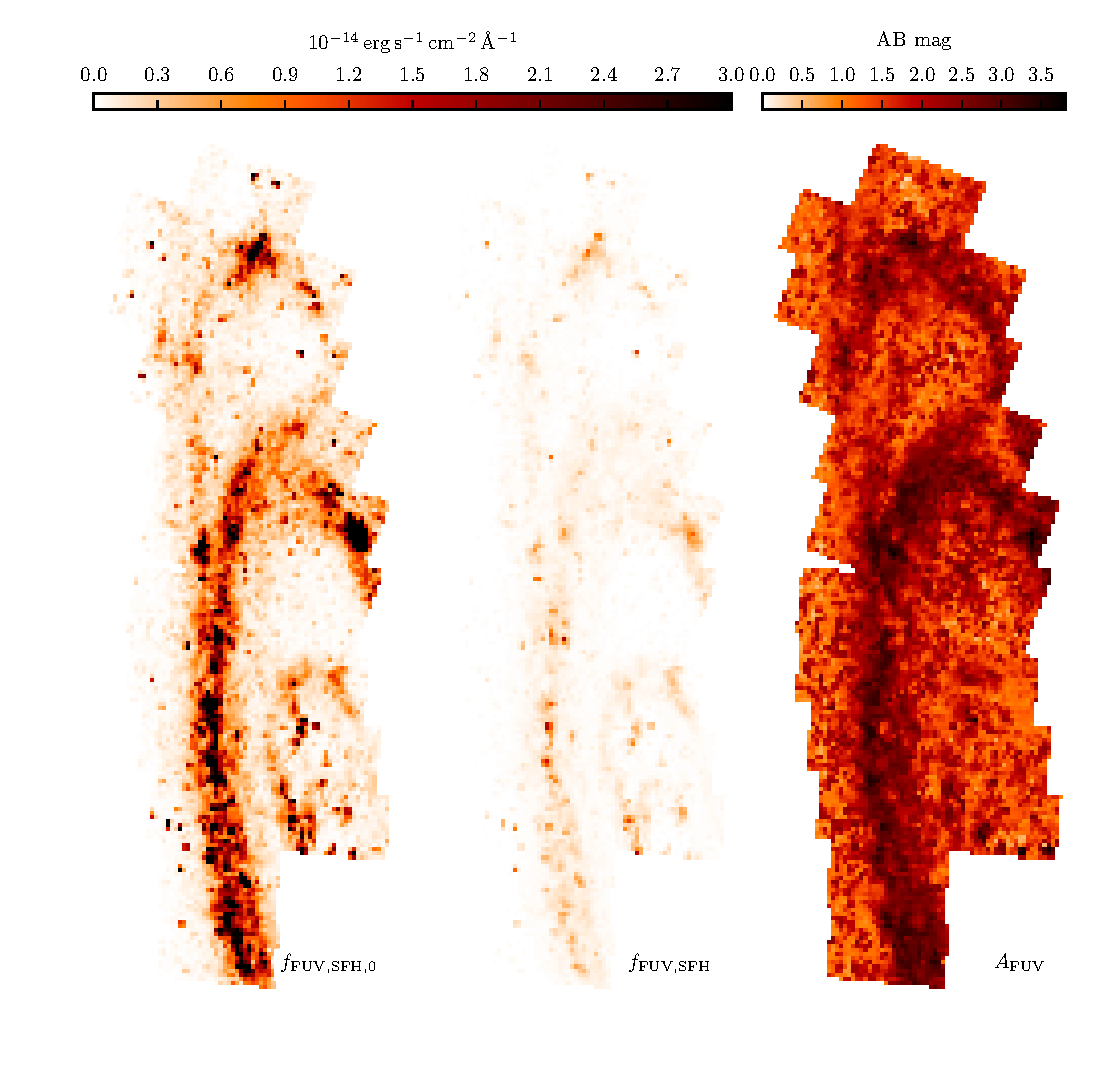
\includegraphics[width=\textwidth]{m31flux-figures/modfluxmaps_fuv.pdf}
\caption[\fuv{} flux map modeled from the SFHs.]{\fuv{} flux modeled from the SFHs.
    The intrinsic flux, \ffuvsfhz{}, is shown in the left panel and the middle
    panel shows the flux attenuated according to the extinction model, \ffuvsfh{}
    (also shown alongside the observed GALEX \fuv{} flux in Figure
    \ref{fig:mfx:fluxmaps_fuv}). The \fuv{} extinction, \afuv{}, derived from
    \ffuvsfhz{} and \ffuvsfh{} is shown on the right.
}
\label{fig:mfx:modfluxmaps_fuv}
\end{figure*}


% Figure 3
\begin{figure*}
\centering
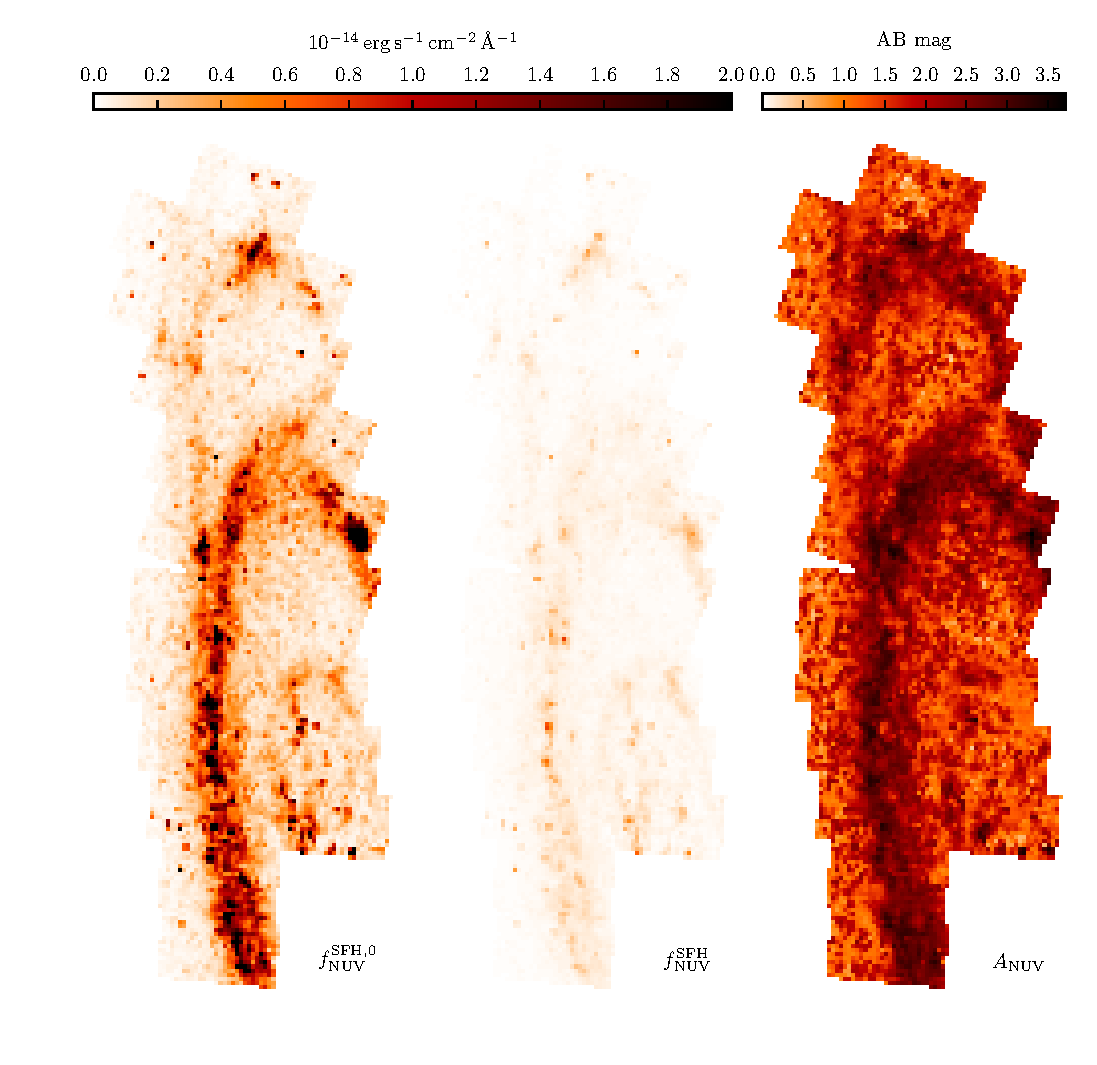
\includegraphics[width=\textwidth]{m31flux-figures/modfluxmaps_nuv.pdf}
\caption[\nuv{} flux map modeled from the SFHs.]{Same as Figure
    \ref{fig:mfx:modfluxmaps_fuv}, but for the \nuv{} filter.
}
\label{fig:mfx:modfluxmaps_nuv}
\end{figure*}


We derived an attenuated SED for the region using the same two-component
extinction model used by MATCH to fit the CMD together with the region's
best-fit \avf{} and \dav{} parameters \citep{Lewis:2014}. To do this, we
divided the intrinsic SED into 30 identical component SEDs (larger numbers of
components did not significantly improve the accuracy of our results). Each
component was attenuated according to the \citet{Cardelli:1989} extinction
curve with a uniform random $A_\mathrm{V}$ drawn between \avf{} and $\avf +
\dav$. The \citet{Cardelli:1989} extinction curve predicts the amount of
extinction relative to that in the V band, $A_\mathrm{V}$, as a function of
wavelength and is based on the average extinction in the Galaxy with a
total-to-selective extinction ratio of $\rv = 3.1$. Previous studies have shown
that this extinction curve is overall applicable to M31 in both the UV
\citep{Bianchi:1996} and the optical \citep{Barmby:2000} regimes. Finally, the
attenuated SED components were summed back together to obtain the region's
integrated attenuated model SED.

The intrinsic and attenuated model SEDs were convolved with the response curves
for the GALEX \fuv{} and \nuv{} filters to obtain absolute synthetic \fuv{} and
\nuv{} magnitudes. These were converted into apparent magnitudes for the region
by projecting to a distance modulus of 24.47 \citep{McConnachie:2005},
consistent with \citet{Lewis:2014}. We used the apparent magnitudes and the
appropriate magnitude-to-flux conversion formulae (see Table
\ref{tab:mfx:filters}) to derive the intrinsic and attenuated broadband UV
fluxes for the region. Hereafter, we will use a subscript (indicated here by
\filter{}) to refer to either \fuv{} or \nuv{} and denote their intrinsic and
attenuated fluxes by \fxsfhz{} and \fxsfh{}, respectively.

After modeling the intrinsic and attenuated fluxes for all of the regions in a
brick, we assembled the flux values (for a given filter) into a $15 \times 30$
array to form an image mapping the synthetic flux across the brick. The brick
map was independently tied to a world coordinate system using a 2D
least-squares optimization to find the best-fit CD matrix
\citep{Calabretta:2002} for a gnomonic tangent plane projection using the known
RA and dec coordinates of the brick grid vertices measured by
\citet{Lewis:2014}. We repeated this process for all of the \citet{Lewis:2014}
bricks, resulting in a set of 21 brick maps. We then reprojected and added the
brick maps using Montage\footnote{http://montage.ipac.caltech.edu/} to create
full maps, or mosaics, of synthetic \fuv{} and \nuv{} flux for the PHAT survey
area.

All of the mosaic maps are registered to a grid defined by a template header
that was automatically chosen by Montage as the best fit to the collection of
input brick maps. The mosaic grid has a pixel scale of $23.75\aarcsec$, which
is comparable to the sizes of the regions from the original brick grids defined
in \citet{Lewis:2014}. Assuming a distance modulus of 24.47
\citep{McConnachie:2005}, a disk inclination of $78\ddeg$ \citep{Tully:1994},
and a major axis position angle of $35\deg$ \citep{deVaucouleurs:1995}, the
pixel scale is deprojected to a linear size of $dx = 440\pc$ and $dy = 100\pc$
approximately along the minor and major axes of M31, respectively. The
synthetic flux maps therefore have a resolution that is firmly in the sub-kpc
regime.

The final synthetic flux maps, \fxsfhz{} and \fxsfh{}, are shown in Figures
\ref{fig:mfx:modfluxmaps_fuv} (\fuv{}) and \ref{fig:mfx:modfluxmaps_nuv}
(\nuv{}).

We used the synthetic flux maps to derive maps of \ax{}, the total extinctions
in the \fuv{} and \nuv{} bands. The intrinsic and attenuated flux maps were
converted into AB magnitudes (Table \ref{tab:mfx:filters}), \xsfhz{} and
\xsfh{}. The extinction maps were then calculated as the difference between the
intrinsic and attenuated magnitudes, $\ax = \xsfh - \xsfhz$. We show the
synthetic extinction maps with their corresponding synthetic flux maps in
Figures \ref{fig:mfx:modfluxmaps_fuv} and \ref{fig:mfx:modfluxmaps_nuv}.

A pixel weight map representing the coverage of the available PHAT data was
also produced during the mosaicking process. Mosaic pixels fully within the
PHAT survey border (excluding bricks 1 and 2 near the bulge) have a weight of
1, pixels fully outside the border have a weight of 0, and all other pixels
have weights between 0 and 1 depending on the fraction of the pixel area within
the survey border. Throughout this study we used the weight map to mask out all
pixels not fully within the survey border so that our comparisons with
observations are done on a full-pixel basis.

%\textbf{*** TODO}
%
%\begin{enumerate}
%\item Uncertainties? The SFHs have statistical uncertainties from the CMD
%    fitting process due to imperfect knowledge of the true underlying SFH that
%    produced the observed CMD. There are also systematic uncertainties due to
%    the optimization of \avf{} and \dav{}. Do we propagate these through to the
%    modeled fluxes, or do we only care about the observational uncertainties
%    (such as in Bayesian analyses where we evaluate the probability of the
%    model given the data and its uncertainties)?
%\item Make sure to add a footnote somewhere indicating that FITS files for the
%    synthetic flux maps, and all of the other maps in this paper, are hosted on
%    github.
%\end{enumerate}
%
%\textbf{***}





\section{Observations}\label{mfx:observations}


% Figure 4
\begin{figure*}
\centering
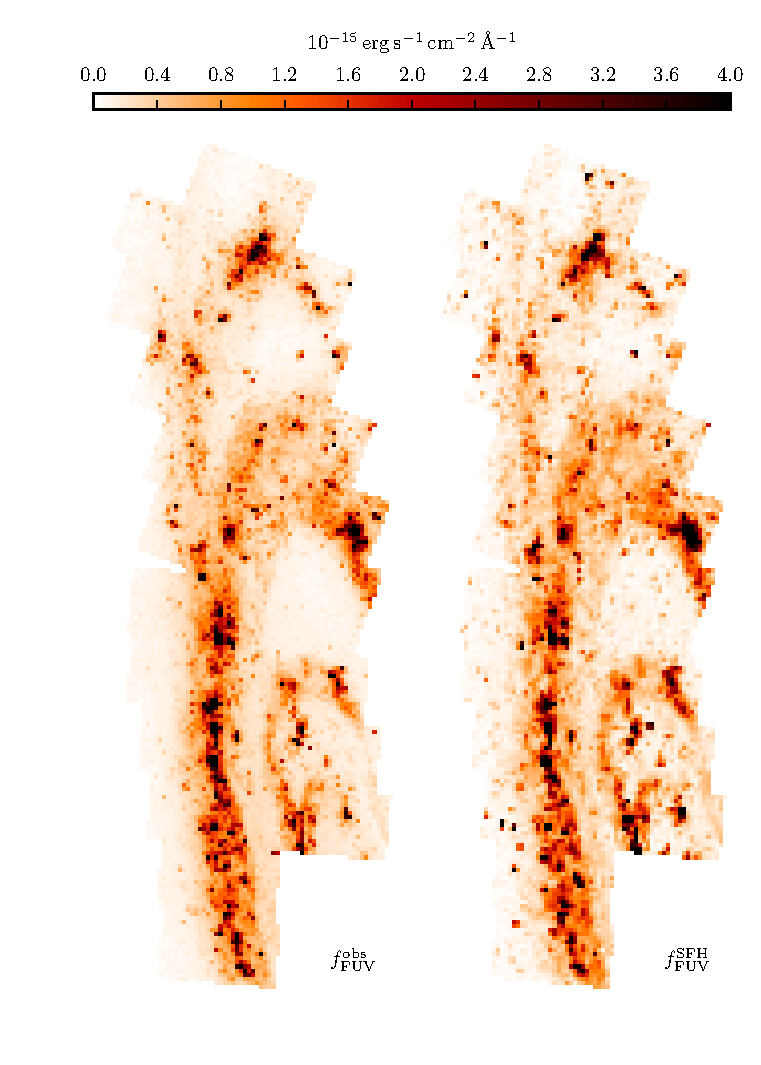
\includegraphics[scale=0.9]{m31flux-figures/fluxmaps_fuv.pdf}
\caption[Observed and synthetic attenuated \fuv{} flux maps.]{Observed \fuv{} flux from
    GALEX, \ffuvobs{} (left), and synthetic attenuated \fuv{} flux from the
    SFHs, \ffuvsfh{} (right). The observed map has been clipped to the PHAT
    survey border to match the synthetic map. The synthetic fluxes show
    excellent morphological agreement with the observed fluxes.
}
\label{fig:mfx:fluxmaps_fuv}
\end{figure*}


% Figure 5
\begin{figure*}
\centering
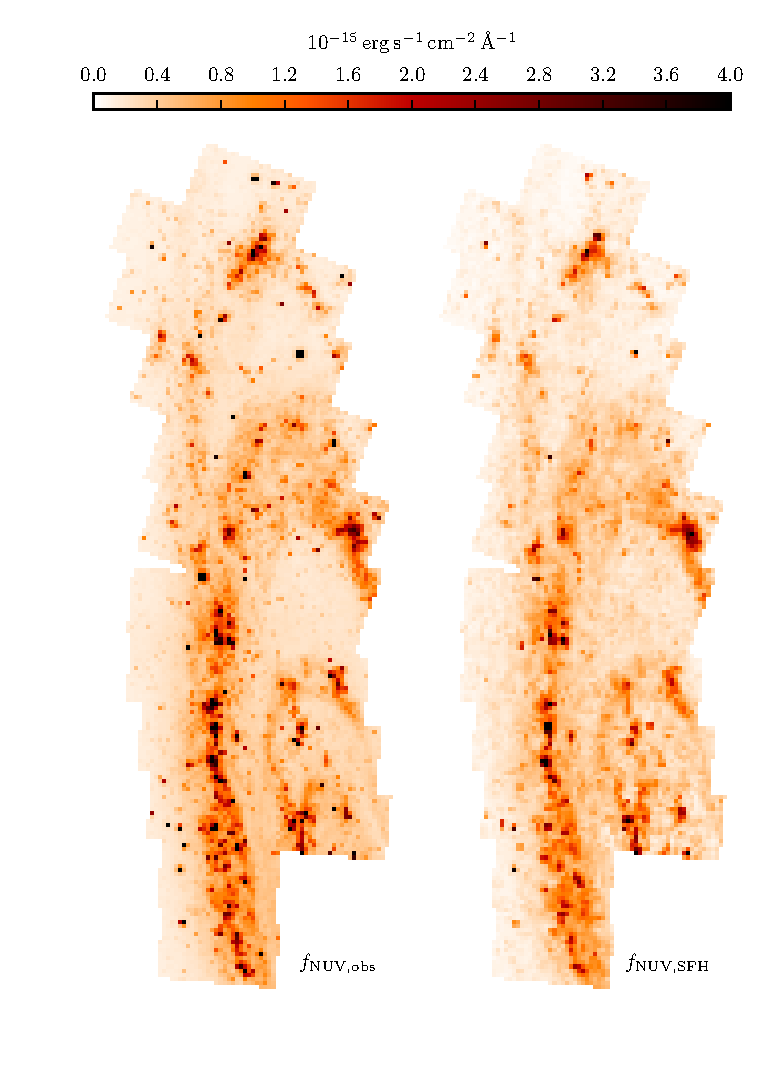
\includegraphics[scale=0.9]{m31flux-figures/fluxmaps_nuv.pdf}
\caption[Observed and synthetic attenuated \nuv{} flux maps.]{Same as Figure
    \ref{fig:mfx:fluxmaps_fuv}, but for the \nuv{} filter.
}
\label{fig:mfx:fluxmaps_nuv}
\end{figure*}


We constructed maps of observed GALEX \fuv{} and \nuv{} flux, \fxobs{}, to
match the synthetic flux maps described in \S
\ref{mfx:syntheticfluxmaps:fluxmod}. We started with the intensity maps of four
tiles in the GALEX Deep Imaging Survey \citep[DIS][]{Martin:2005} covering the
PHAT survey area (see Table \ref{tab:mfx:filters}). The tiles were converted
from units of $\mathrm{counts} \ssec^{-1} \,\mathrm{pixel}^{-1}$ into flux
using the factors in Table \ref{tab:mfx:filters}. We then used Montage to
reproject the flux tiles to the same template header as the synthetic flux
mosaics (see \S \ref{mfx:syntheticfluxmaps}). The individual tiles had slightly
different background levels, so we had Montage automatically match the
backgrounds before adding the tiles to form the final mosaic.

A small amount of background UV flux was present in the \fuv{} and \nuv{}
mosaics, primarily due to scattering of UV photons from hot foreground stars in
the Galaxy. We measured the mean background flux in a rectangular aperture in
an off-galaxy area relatively devoid of stars in the reprojected, background
matched tile PS\_M31\_MOS07. The measured background values were $5.22 \times
10^{-19}$ and $3.47 \times 10^{-19}\uflambda\aarcsec^{-2}$ ($2.9 \times
10^{-16}$ and $2.0 \times 10^{-16}\uflambda$ per mosaic pixel) in \fuv{} and
\nuv{}, respectively. We subtracted these values from the \fuv{} and \nuv{}
mosaics to obtain the final observed UV flux maps for the PHAT survey area,
\fxobs{}, shown in Figures \ref{fig:mfx:fluxmaps_fuv} (\fuv{}) and Figure
\ref{fig:mfx:fluxmaps_nuv} (\nuv{}).

%\textbf{*** TODO}
%
%\begin{enumerate}
%\item Uncertainties? For statistical/Poisson uncertainties, divide the \fuv{}
%    and \nuv{} intensity (count) maps by the CCD gain to convert the units into
%    photons, and take the square root. Flux is proportional to photon rate, so
%    the flux uncertainties are just a constant times the raw Poisson
%    uncertainties. The uncertainties won't be useful for the map
%    visualizations, but they will be important for scatter plots comparing the
%    synthetic and observed fluxes.
%\end{enumerate}
%
%\textbf{***}





\section{SFR estimates}\label{mfx:sfrestimates}


% Figure 6
\begin{figure*}
\centering
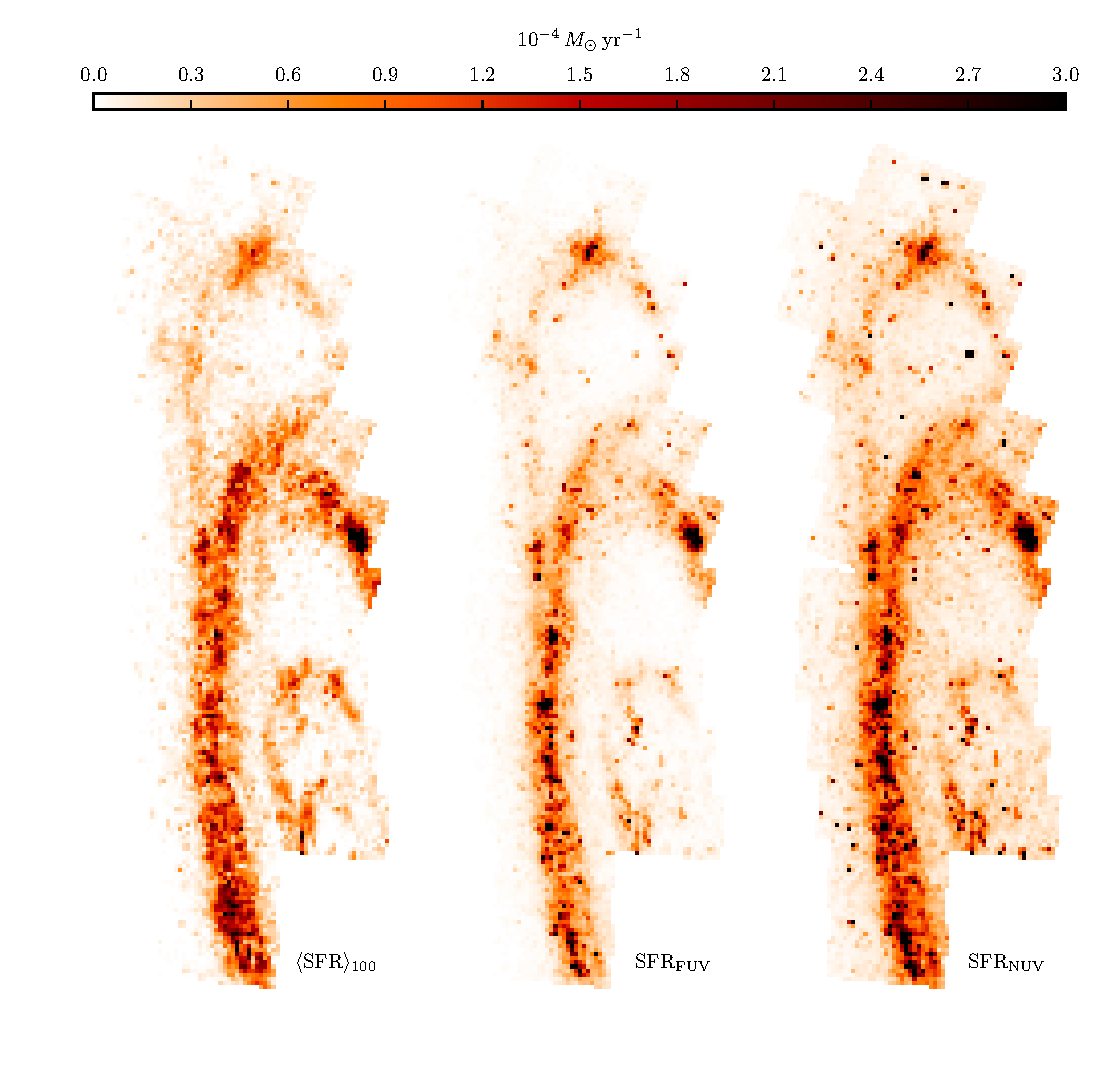
\includegraphics[width=\textwidth]{m31flux-figures/sfrmaps1.pdf}
\caption[SFR maps from estimates based on observed fluxes compared with the
    mean SFR map from the SFHs.]{\fuv{} and \nuv{} flux-based SFRs, \sfrfuv{}
    (middle) and \sfrnuv{} (right), compared with \sfroneh{} (left), the mean
    SFR over the last $100\myr$ of the SFHs. The flux-based SFRs were derived
    from the observed GALEX fluxes, \fuvobs{} and \nuvobs{} (Figures
    \ref{fig:mfx:fluxmaps_fuv} and \ref{fig:mfx:fluxmaps_nuv}), corrected for
    extinction using \afuv{} and \anuv{} (Figures \ref{fig:mfx:modfluxmaps_fuv}
    and \ref{fig:mfx:modfluxmaps_nuv}). The SFR maps show good overall
    agreement.
}
\label{fig:mfx:sfrmaps1}
\end{figure*}


% Figure 7
\begin{figure*}
\centering
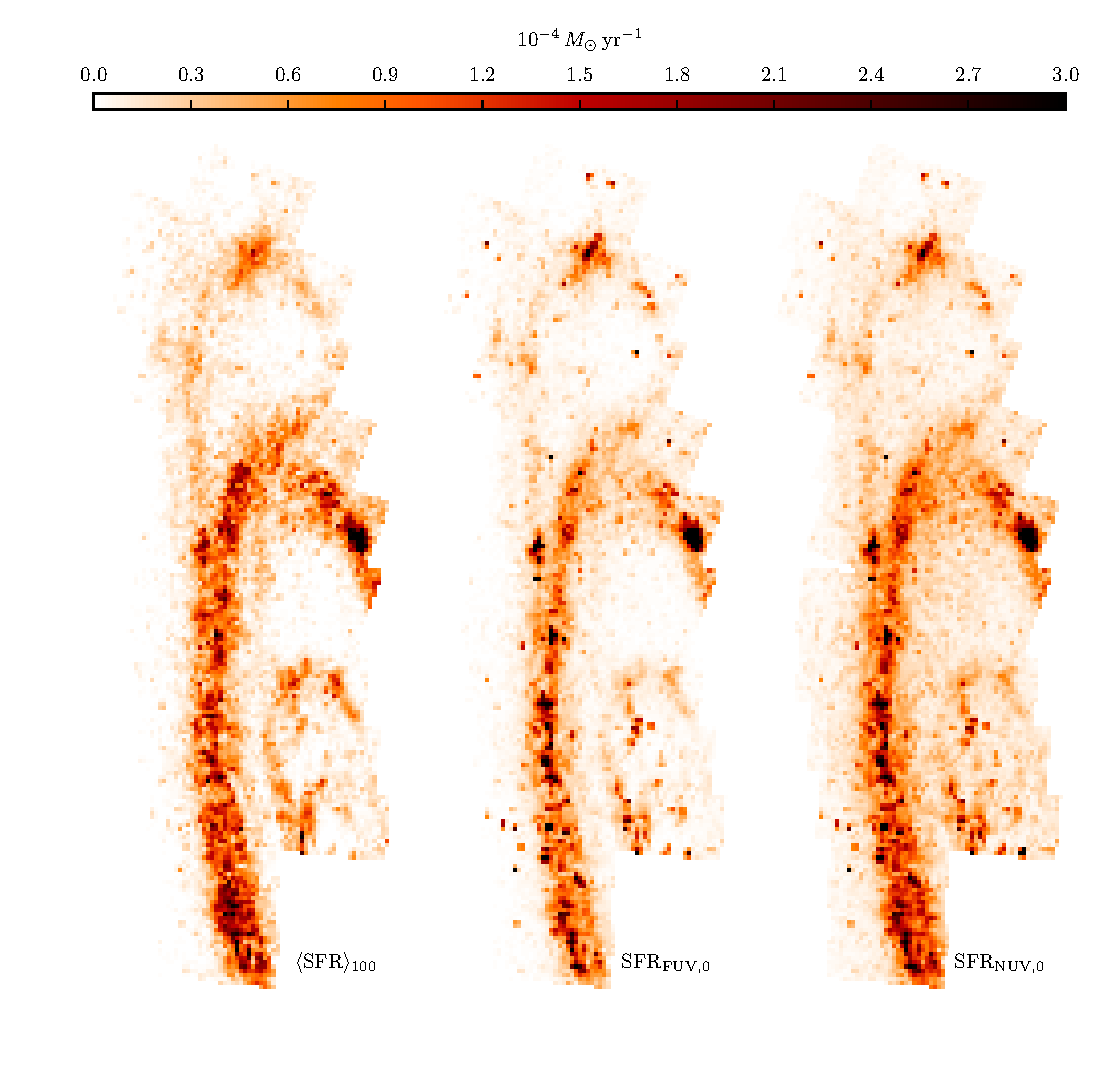
\includegraphics[width=\textwidth]{m31flux-figures/sfrmaps2.pdf}
\caption[SFR maps from estimates based on synthetic intrinsic fluxes compared
    with the mean SFR map from the SFHs.]{Same as Figure
    \ref{fig:mfx:sfrmaps1}, but instead comparing \sfroneh{} with \sfrfuvz{}
    and \sfrnuvz{}, the SFRs from the synthetic intrinsic (i.e., unattenuated)
    fluxes from Figures \ref{fig:mfx:modfluxmaps_fuv} and
    \ref{fig:mfx:modfluxmaps_nuv}. The synthetic intrinsic fluxes were derived
    assuming a fully populated IMF so there is no inconsistency with the flux
    calibration, which assumes the same. Like the SFRs based on observed flux,
    these SFRs also show good agreement with \sfroneh{}.
}
\label{fig:mfx:sfrmaps2}
\end{figure*}


A common method for estimating the SFR of a target is to measure the integrated
flux in one or more filters and then calculate the SFR using one of the
flux-to-SFR calibrations available in the literature, e.g., (for UV flux) those
discussed by \citet{Kennicutt:1998}, \citet{Salim:2007}, \citet{Hao:2011},
\citet{Murphy:2011}, and \citet{Leroy:2012}; see also the review by
\citet{Kennicutt:2012}. We used this method to derive SFR maps for the PHAT
survey area, which we can later compare with similar maps derived from the
\citet{Lewis:2014} SFH data, effectively extending the work of
\citet{Simones:2014} to a much larger and more diverse sample.

To calculate flux-based SFRs, we converted the \fxobs{} maps into AB magnitudes
(Table \ref{tab:mfx:filters}), \xobs{}, which we corrected for extinction by
subtracting the synthetic \ax{} maps (\S \ref{mfx:syntheticfluxmaps:fluxmod}).
The extinction-corrected maps were converted back into (specific) fluxes ($\erg
\ssec^{-1} \cm^{-2} \ang^{-1}$), then into total fluxes ($\erg \ssec^{-1}
\cm^{-2}$) by multiplying by the effective filter wavelength
\citep[$1538.6\ang$ for \fuv{}, $2315.7\ang$ for \nuv{};][]{Morrissey:2007}.
The total fluxes were converted into luminosities, \lx{} ($\erg \ssec^{-1}$),
assuming a distance modulus of 24.47 \citep{McConnachie:2005}. Finally, we
applied the calibrations from \citet{Kennicutt:1998} with updates by
\citet{Hao:2011} and \citet{Murphy:2011} \citep[see the review
by][]{Kennicutt:2012} to obtain the \fuv{} and \nuv{} flux-based SFR estimates,
\sfrx{}, respectively:
\begin{equation}
\left(\frac{\sfrfuv}{\msun\yr^{-1}}\right) =
    10^{-43.35}\,\left(\frac{\lfuv}{\erg\ssec^{-1}}\right)
\label{mfx:eq:fuvcal}
\end{equation}
\begin{equation}
\left(\frac{\sfrnuv}{\msun\yr^{-1}}\right) =
    10^{-43.17}\,\left(\frac{\lnuv}{\erg\ssec^{-1}}\right)
\label{mfx:eq:nuvcal}
\end{equation}
These calibrations are based on stellar population synthesis using Starburst99
\citep{Leitherer:1999} and assuming a constant SFR over the last $100\myr$, the
\citet{Kroupa:2001} IMF, a fully populated range of masses from 0.1 to
$100\msun$, and solar metallicity \citep{Hao:2011}.

The most robust flux calibrations are the those that rely on more than one part
of the electromagnetic spectrum. An example of a hybrid estimator is the
combination of GALEX \fuv{} and Spitzer $24\,\mu\mathrm{m}$ fluxes, which
simultaneously accounts for the direct starlight from newly-formed massive
stars and the absorbed starlight processed and reradiated by dust
\citep[e.g.,][]{Leroy:2012}. However, we have limited our study to observations
by GALEX, so we will only consider the simpler monochromatic \fuv{} and \nuv{}
calibrations in Equations \ref{mfx:eq:fuvcal} and \ref{mfx:eq:nuvcal}. We show
the final \sfrx{} maps in Figure \ref{fig:mfx:sfrmaps1}.

We also created a map for the mean SFR over the past $100\myr$ of the SFHs,
\sfroneh{}, which we show alongside the flux-based SFR maps in Figure
\ref{fig:mfx:sfrmaps1}. The $100\myr$ limit represents the nominal timescale of
UV emission and matches the timescale used by \citet{Hao:2011} to derive the
\fuv{} and \nuv{} flux calibrations.

Finally, we created another pair of flux-based SFR maps derived just as before,
except instead we started with the intrinsic synthetic fluxes \fxsfhz{}
described in \S \ref{mfx:syntheticfluxmaps:fluxmod}. Because the fluxes were
intrinsic, it was not necessary to apply an extinction correction before
converting the fluxes into SFRs. The maps for the intrinsic flux-based SFR
estimates, \sfrxz{}, are shown in Figure \ref{fig:mfx:sfrmaps2}.




\section{Discussion}\label{mfx:discussion}



\subsection{Modeled flux}\label{mfx:discussion:modflux}

Figures \ref{fig:mfx:fluxmaps_fuv} and \ref{fig:mfx:fluxmaps_nuv} show
remarkable overall qualitative agreement between the synthetic attenuated
fluxes \fxsfh{} and the observed GALEX fluxes \fxobs{}. In particular, all of
the main features brighter than $\sim 10^{-15}\uflambda$ in the observed maps
are faithfully reproduced in the synthetic maps. This includes the main rings
at $\sim 5$, 10, and $15\kpc$ from the bulge, and the large star-forming
complexes found in PHAT bricks 15 and 21. The \fnuvobs{} map does show several
point sources (most likely foreground stars) which are not present in the
\fnuvsfh{} map, but the synthetic maps were derived to simulate fluxes from
\emph{distributions} of stars in CMDs, not the stars individually.

We compare the synthetic and observed fluxes more quantitatively in Figures
\ref{fig:mfx:fuvfluxratio} (\fuv{}) and \ref{fig:mfx:nuvfluxratio} (\nuv{}),
which map the ratio of \fxsfh{} to \fxobs{} over the PHAT survey area. The
Figures also show the flux ratios as a function of \fxobs{}. We find that the
log flux ratios follow normal distributions with mean $\mu = 7.62\times
10^{-3}$ and standard deviation $\sigma = 2.37\times 10^{-1}$ for \fuv{}, and
$\mu = -1.03\times 10^{-1}$ and $\sigma = 1.59\times 10^{-1}$ for \nuv{}. In
linear terms, the median flux ratios are 1.02 in \fuv{} and 0.79 in \nuv{},
with 68\% confidence limits of 0.59 and 1.76 (\fuv{}) and 0.55 and 1.14
(\nuv{}). Note that in both filters, the median ratio is within the confidence
interval of 1, indicating that \fxsfh{} is consistent with \fxobs{} on average.


% Figure 8
\begin{figure*}
\centering
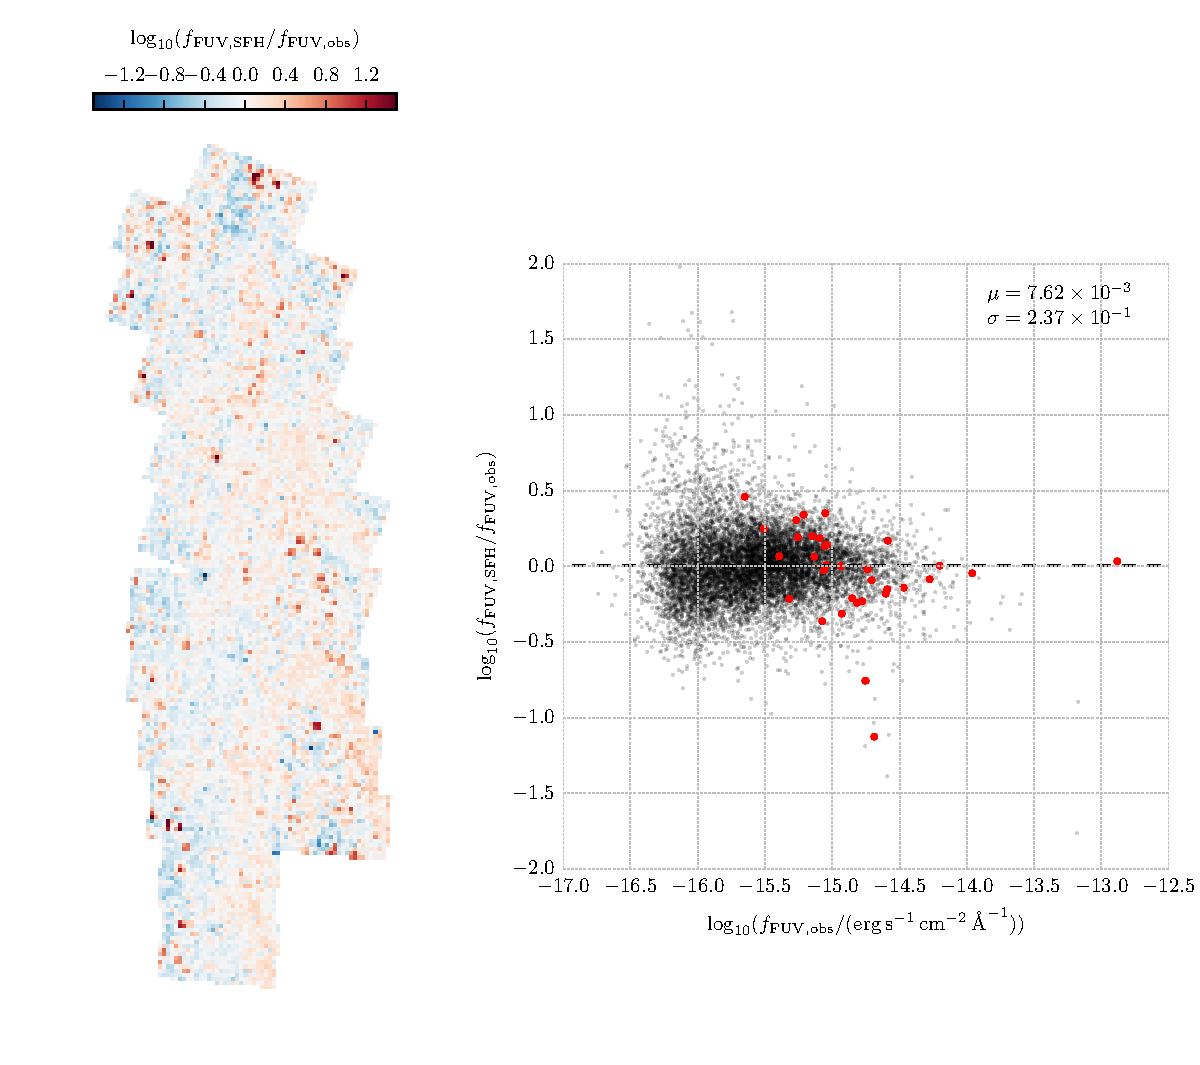
\includegraphics[width=\textwidth]{m31flux-figures/flux_fuv_sfh-vs-obs.pdf}
\caption[Ratio of the synthetic flux to the observed flux in the \fuv{}
filter.]{Ratio of the synthetic attenuated flux, \ffuvsfh{}, to the GALEX
    observed flux, \ffuvobs{}, in the \fuv{} filter. The log flux ratios in the
    scatter plot follow a normal distribution with $\mu = 7.62\times 10^{-3}$
    (horizontal dashed line) and $\sigma = 2.37\times 10^{-1}$. The median
    ratio is 1.02 with 68\% confidence limits of 0.59 and 1.76. \ffuvsfh{} and
    \ffuvobs{} are therefore consistent on average. The flux ratio variance
    increases with decreasing observed flux, suggesting that the uncertainties
    are dominated by incomplete IMF sampling. The large red circles represent
    flux ratios for the UV-bright regions from \citet{Simones:2014} and are
    consistent with the main sample. The map shows a fairly even spatial
    distribution for the flux ratios, with the most severely overestimated and
    underestimated pixels occurring primarily in the faint, off-arm areas of
    the galaxy, as shown in the scatter plot.
}
\label{fig:mfx:fuvfluxratio}
\end{figure*}


% Figure 9
\begin{figure*}
\centering
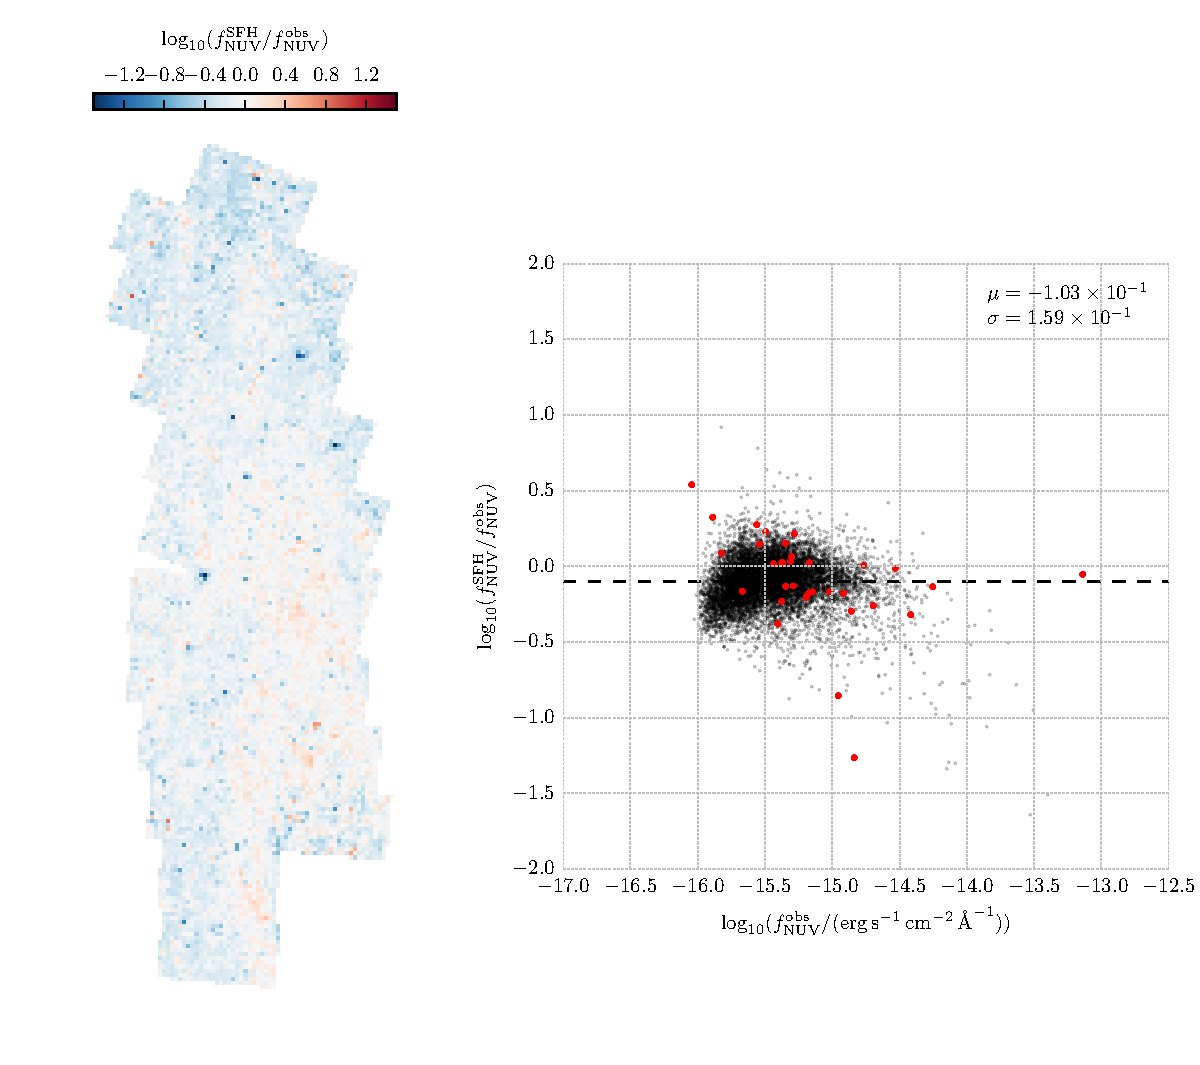
\includegraphics[width=\textwidth]{m31flux-figures/flux_nuv_sfh-vs-obs.pdf}
\caption[Ratio of the synthetic flux to the observed flux in the \nuv{}
filter.]{Same as Figure \ref{fig:mfx:fuvfluxratio}, but for the \nuv{} filter.
    In this case, the log-normal distribution is characterized by $\mu =
    -1.03\times 10^{-1}$ and $\sigma = 1.59\times 10^{-1}$. The median ratio is
    0.79 with 68\% confidence limits of 0.55 and 1.14. \fnuvsfh{} and
    \fnuvobs{} are therefore consistent on average. The role of IMF sampling is
    not as important for \fnuvobs{}, so the uncertainties in \fnuvsfh{} are
    somewhat smaller.
}
\label{fig:mfx:nuvfluxratio}
\end{figure*}


The overall agreement between \fxsfh{} and \fxobs{} shows that our modeling
procedure is generally robust and justifies the several key assumptions that we
and \citet{Lewis:2014} used to derive \fxsfh{} from the CMDs. Specifically, we
assumed an IMF, models describing stellar spectra and evolution, and an
extinction model as well as an extinction curve. These form the foundation for
much research in astronomy and encompass our current best understanding of
stellar astrophysics and star formation. It is therefore reassuring that we can
use all of this knowledge to derive SFHs, synthesize SEDs, and successfully
recreate detailed maps of a galaxy, all from photometry in just two optical
bands.

The Poisson uncertainties in \fxobs{} are relatively small. Assuming an average
exposure time of $7\times 10^3\ssec$ in the \fuv{} channel for the five DIS
images in our study, the uncertainties are only a few percent at $\ffuvobs \sim
10^{-16}\uflambda$ and a few tenths of a percent at $\ffuvobs \sim
10^{-14}\uflambda$. The corresponding \nuv{} uncertainties for an average
exposure time of $6\times 10^4\ssec$ in the \nuv{} channel are about one tenth
of those in the \fuv{}. However, Figures \ref{fig:mfx:fuvfluxratio} and
\ref{fig:mfx:nuvfluxratio} show variances that are much larger than the Poisson
uncertainties allow. These variances are therefore due essentially exclusively
to systematic effects in the modeling process.

The primary systematic effect at play is most likely incomplete sampling of the
IMF
\citep{Elmegreen:1999,Bastian:2010,Fumagalli:2011,daSilva:2012,daSilva:2014}.
This is supported by the observation that the variance in the flux ratios
increases with decreasing pixel brightness, especially in the \fuv{} filter.
Also, the \fxsfh{} maps show somewhat more uneven, noisy backgrounds, i.e.,
faint pixels in the off-arm areas of M31, compared with the \fxobs{} maps. The
faint pixels are associated with low star formation (SF) activity and, because
all pixels are the same size, have fewer stars than the brighter pixels
covering the arms and main star-forming regions. This leads to a violation of
the full-IMF assumption used by FSPS and other stellar population synthesis
codes.

Whenever the number of stars in a population is sufficiently small, the
discreteness of the stellar mass distribution becomes important in determining
the observed luminosity compared with other populations of the same total mass.
This is because any given sampling of the total mass can easily have a higher
(or lower) proportion of high-mass stars than expected for a fully populated
IMF. There will therefore be more (or less) high-energy photons than stellar
population synthesis models suggest, and the synthetic UV flux will be
underestimated (or overestimated). In other words, when a stellar population is
small, the same total mass could be produced by a variety of mass functions
(samplings of the IMF), where each mass function has its own unique luminosity.
This results in a variance in the flux ratios that increases with decreasing
surface brightness. We observe this trend to be more pronounced in \fuv{}, as
mentioned above, and is caused by the increased sensitivity of \ffuvobs{} to
slight variations in the number of high-mass stars relative to \fnuvobs{}.

Although IMF sampling more severely affects the fainter pixels, the sub-kpc
resolution of our flux maps results in small pixel areas such that IMF sampling
is likely the dominant source of the variance for all of the flux ratios.
Accounting for projection effects in the disk, the physical area of each pixel
is $4.4\times 10^4\pc^2$ (\S \ref{mfx:syntheticfluxmaps:fluxmod}). This is
approximately equal to the average area of the UV-bright regions considered by
\citet{Simones:2014}, who showed that the uncertainties in fluxes modeled for
UV-bright regions tapers off with increasing area. They also showed that
combining several small regions into a larger $\sim\kpc$-sized region greatly
improved the agreement between the synthetic and observed fluxes. These results
show that the best way to comply with the full-IMF assumption and reduce the
uncertainties in \fxsfh{} is to make the mosaic pixel size larger. Naturally,
reducing uncertainties this way comes at the cost of decreased spatial
resolution in the flux maps. Exploring simultaneously the effects of both
surface brightness \emph{and} pixel area on this fundamental, stochastic
variance is an interesting topic for future study.

We have added to Figures \ref{fig:mfx:fuvfluxratio} and
\ref{fig:mfx:nuvfluxratio} the flux ratios for the sample of UV-bright regions
in \citet{Simones:2014}. Although the UV-bright regions vary in size and come
from one small part of M31, their flux ratios appear to agree with the overall
distribution for the rest of the galaxy. Also, other than the increased
variance in the faint areas, we find no obvious trends in the mean or variance
of the flux ratios with respect to environment or distance from the bulge.
Therefore, we conclude that the flux modeling procedure may be successfully
applied to any population in environments similar to M31. We estimate the
uncertainties in synthesizing fluxes for sub-kpc regions to be $+\!0.74/\!-\!0.43$
and $+\!0.35/\!-\!0.24$ times the observed flux in \fuv{} and \nuv{}, respectively,
driven mostly by incomplete sampling of the IMF. The \ffuvsfh{} uncertainties
are consistent with \citet{Simones:2014}, who found an uncertainties of
$+\!0.95/\!-\!0.47$ for the synthetic \fuv{} fluxes of the UV-bright regions.



\subsection{SFR estimates from FUV flux}


% Figure 10
\begin{figure*}
\centering
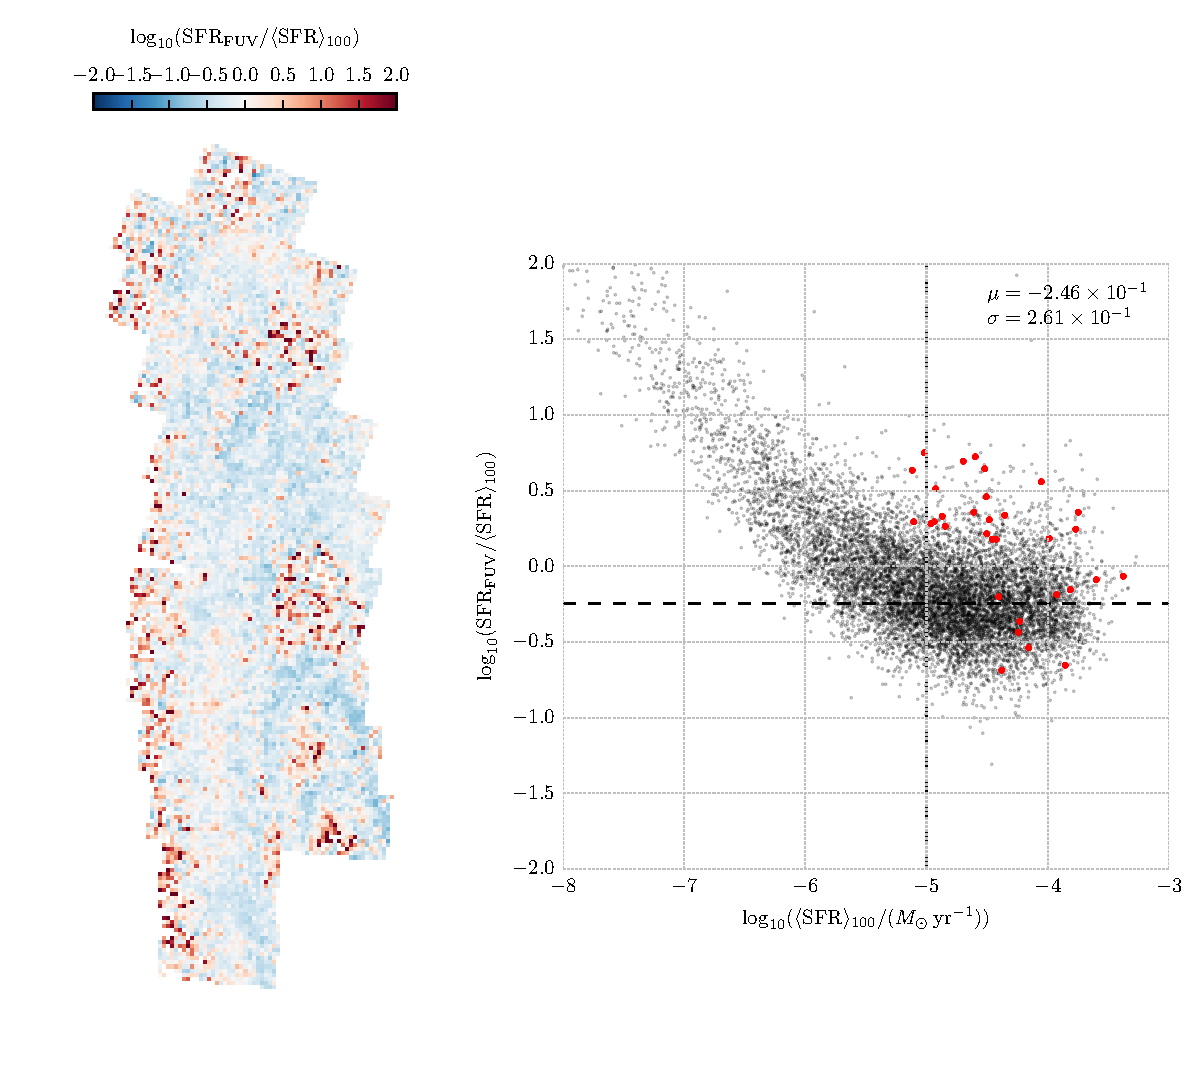
\includegraphics[width=\textwidth]{m31flux-figures/sfr_fuv-vs-mean.pdf}
\caption[Ratio of the \sfr{} based on the observed extinction-corrected \fuv{}
flux to the $100\myr$ mean \sfr{}.]{Ratio of the \sfr{} based on the observed
    extinction-corrected \fuv{} flux, \sfrfuv{}, to the $100\myr$ mean of the
    SFH, \sfroneh{}. The log SFR ratios show a linear tail feature with $-1$
    slope and $-6.0$ intercept, implying that \sfrfuv{} becomes constant for
    $\sfroneh < 9.8\times 10^{-7}\msun\yr^{-1}$. We constrain our analysis to
    pixels with $\sfroneh10^{-5}\msun\yr^{-1}$ (vertical dashed line). Above
    this limit, the log SFR ratios follow a normal distribution with $\mu =
    -2.46\times 10^{-1}$ (horizontal dashed line) and $\sigma = 2.61\times
    10^{-1}$. The median ratio is 0.57 with 68\% confidence limits of 0.31 and
    1.04, most likely due to incomplete IMF sampling. \sfrfuv{} and \sfroneh{}
    are therefore consistent on average. The large red circles represent SFR
    ratios for the UV-bright regions from \citet{Simones:2014} and are
    consistent with the main sample. Apart from the faint, off-arm areas
    responsible for the tail feature, the map shows a fairly even spatial
    distribution for the SFR ratios.
}
\label{fig:mfx:fuvsfrratio}
\end{figure*}


% Figure 11
\begin{figure*}
\centering
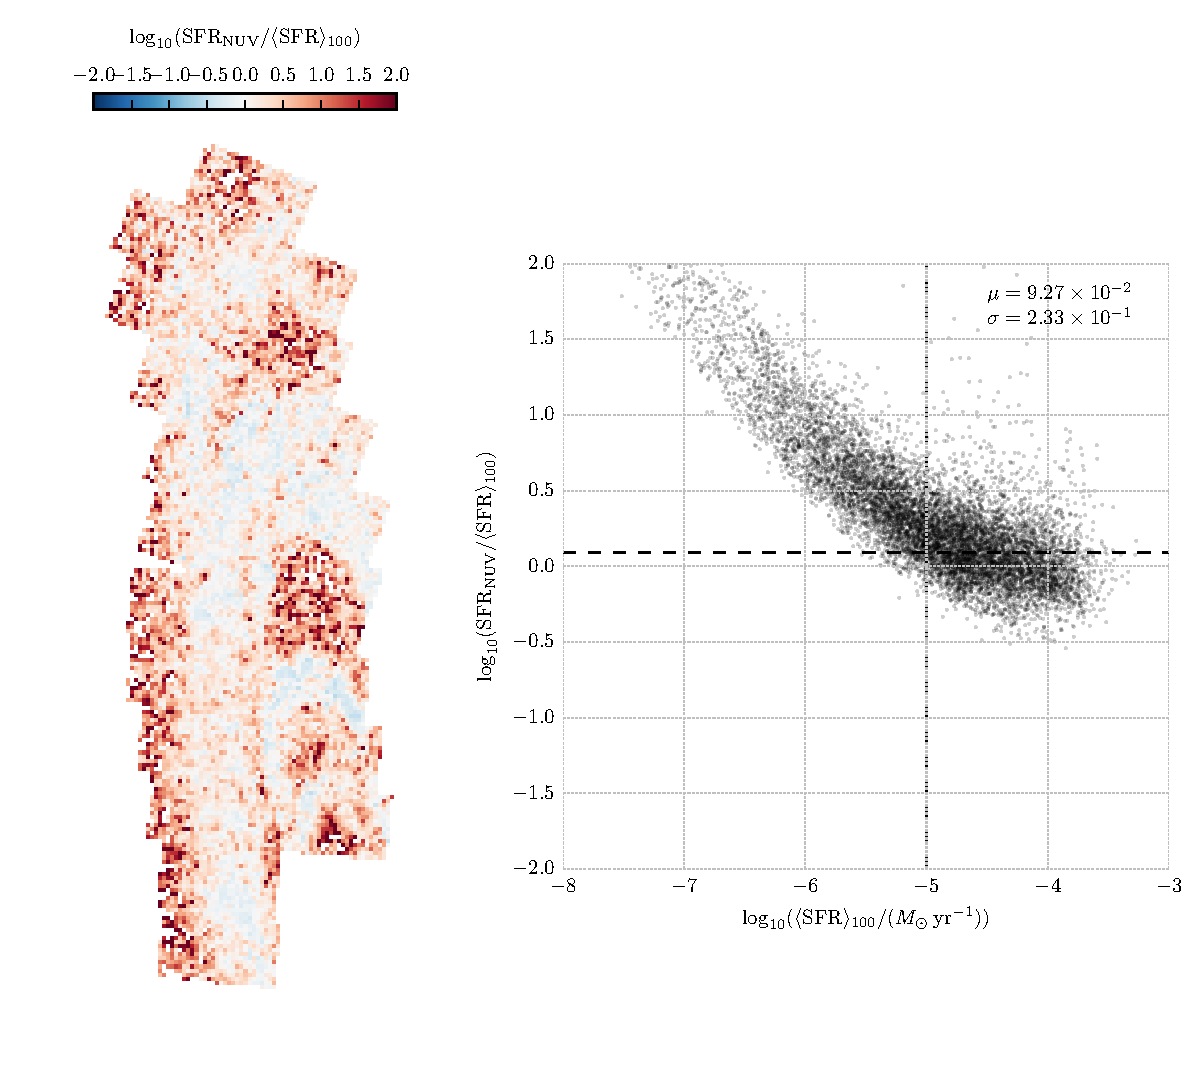
\includegraphics[width=\textwidth]{m31flux-figures/sfr_nuv-vs-mean.pdf}
\caption[Ratio of the \sfr{} based on the observed extinction-corrected \nuv{}
flux to the $100\myr$ mean \sfr{}.]{Same as Figure \ref{fig:mfx:fuvsfrratio},
    but for the \nuv{} filter. In this case, the linear tail has an intercept
    of $-5.4$ such that \sfrnuv{} becomes constant for $\sfroneh < 4.1\times
    10^{-6}\msun\yr^{-1}$. The log-normal distribution is characterized by $\mu
    = 9.27\times 10^{-2}$ and $\sigma = 2.33\times 10^{-1}$. The median ratio
    is 1.24 with 68\% confidence limits of 0.72 and 2.12. \sfrnuv{} and
    \sfroneh{} are therefore consistent on average.
}
\label{fig:mfx:nuvsfrratio}
\end{figure*}


As with the synthetic and observed fluxes, the flux-based SFR maps in Figures
\ref{fig:mfx:sfrmaps1} and \ref{fig:mfx:sfrmaps2} show good overall
morphological agreement with the \sfroneh{} map. We compare the SFRs more
closely in Figures \ref{fig:mfx:fuvsfrratio} and \ref{fig:mfx:nuvsfrratio}, in
which we map the ratio of \sfrx{} to \sfroneh{} and plot the SFR ratio as a
function of \sfroneh{}. A major feature in both figures is the marked contrast
in the SFR ratios between the high and low SFR areas. The areas with low
\sfroneh{}, corresponding to the faint areas in Figures
\ref{fig:mfx:fluxmaps_fuv} and \ref{fig:mfx:fluxmaps_nuv}, host nearly all of
the very highest SFR ratios in the entire survey area and none of the low or
moderate ratios. The pixels in these areas make up the downward sloping tails
seen at low \sfroneh{} in the scatter plots in Figures \ref{fig:mfx:sfrmaps1}
and \ref{fig:mfx:sfrmaps2}.

The low-SFR tails are distinctly linear, with slopes of $-1$ and intercepts of
$-6.0$ and $-5.4$ for the \fuv{} and \nuv{} SFR ratios, respectively. In log
space, a straight line with $-1$ slope indicates that \sfrx{} becomes constant
with a value equal to $10^{-6.0} = 9.8\times 10^{-7}\msun\yr^{-1}$ for \fuv{}
and $10^{-5.4} = 4.1\times 10^{-6}\msun\yr^{-1}$ for \nuv{}. Because \sfrx{} is
directly proportional to \fxobs{}, these SFR constants suggest that there must
be a constant baseline flux present in the galaxy that becomes more apparent as
\sfroneh{} decreases to very small values. In other words, the linear
relationship between flux and SFR assumed by the flux calibrations in Equations
\ref{mfx:eq:fuvcal} and \ref{mfx:eq:nuvcal} appear to break down completely
below \sfroneh{} approximately one to a $\mathrm{few} \times
10^{-6}\msun\yr^{-1}$.

Using the flux calibrations in reverse, we find that the above SFR constants
translate into $\ffuvobs \sim 2\times 10^{-16}\uflambda$ and $\fnuvobs \sim
8\times 10^{-16}\uflambda$ (or -15.7 and -15.1 in log flux, respectively). All
of Figures  \ref{fig:mfx:sfrmaps1}, \ref{fig:mfx:sfrmaps2},
\ref{fig:mfx:fuvfluxratio}, and \ref{fig:mfx:nuvfluxratio} show that these flux
and SFR limits make the \fuv{} and \nuv{} flux-to-SFR calibrations completely
unreliable for approximately half of the pixels in the survey area. This
demonstrates the importance of warnings in the literature
\citep[e.g.,][]{Murphy:2011,Kennicutt:2012,Leroy:2012} that flux calibrations
are problematic on sub-kpc scales. We therefore limit our analysis of the SFR
ratios in Figures \ref{fig:mfx:fuvsfrratio} and \ref{fig:mfx:nuvsfrratio} to
pixels with \sfroneh{} greater than a conservative threshold of
$10^{-5}\msun\yr^{-1}$.

Considering only pixels with $\sfroneh \ge 10^{-5}\msun\yr^{-1}$, we treat the
SFR ratios as having log-normal distributions with $\mu = -2.46\times 10^{-1}$
and $\sigma = 2.61\times 10^{-1}$ for \fuv{}, and $\mu = 9.27\times 10^{-2}$
and $\sigma = 2.33\times 10^{-1}$ for \nuv{}. The median ratios are 0.57
(\fuv{}) and 1.24 (\nuv{}), with 68\% confidence limits of 0.31 and 1.04
(\fuv{}) and 0.72 and 2.12 (\nuv{}), indicating that \sfrx{} is consistent with
\sfroneh{} on average. However, given the small uncertainties for the observed
fluxes (\S \ref{mfx:syntheticfluxmaps:fluxmod}) the large variances of the SFR
ratios suggest that significant systematic effects are involved in the
flux-to-SFR conversion process.

One of the assumptions made by the flux calibrations in Equations
\ref{mfx:eq:fuvcal} and \ref{mfx:eq:nuvcal} is that the input flux is produced
by a stellar population with solar metallicity. The mean metallicity of the
brick grid regions (\S \ref{mfx:syntheticfluxmaps:fluxmod}) is $\met = -0.06$
with a standard deviation of 0.09, so the mosaic pixels are consistent with
solar metallicity on average. From \citet{Simones:2014}, overestimating \met{}
by $0.1\dex$ causes the SFR to be overestimated by $0.015\dex$. Therefore, the
variation in the metallicities contributes only $0.01\dex$ to the variation in
the log SFR ratios, making metallicity unimportant for the overall SFR ratio
distribution.

Like the modeled fluxes in \S \ref{mfx:discussion:modflux}, the flux
calibrations also assume a fully populated IMF, causing \sfrx{} to be
overestimated (or underestimated) for pixels with an apparent excess (or lack)
of massive stars. Also, if incomplete IMF sampling is the primary source of the
variance in the log SFR ratios, as it is for the log flux ratios, then the
$\sigma$ parameters of the log-normal distributions should be similar. Indeed,
we find consistent variances between Figures \ref{fig:mfx:fuvfluxratio} and
\ref{fig:mfx:fuvsfrratio} and between Figure \ref{fig:mfx:nuvfluxratio} and
\ref{fig:mfx:nuvsfrratio}.

The flux calibrations also assume a constant SFH over the last 100 Myr. The
analysis of UV-bright regions in \citet{Simones:2014} showed that
inconsistencies with this assumption can contribute at least as much to the
total uncertainty in \sfrfuv{} as incomplete IMF sampling. To isolate the
effect of SFH variability, we recreate in Figures \ref{fig:mfx:fuvzsfrratio}
and \ref{fig:mfx:nuvzsfrratio} the maps and plots of Figures
\ref{fig:mfx:fuvsfrratio} and \ref{fig:mfx:nuvsfrratio} using \sfrxz{}, the
SFRs derived from the synthetic intrinsic fluxes (see \S
\ref{mfx:syntheticfluxmaps:fluxmod}) instead of \sfrx{}.


% Figure 12
\begin{figure*}
\centering
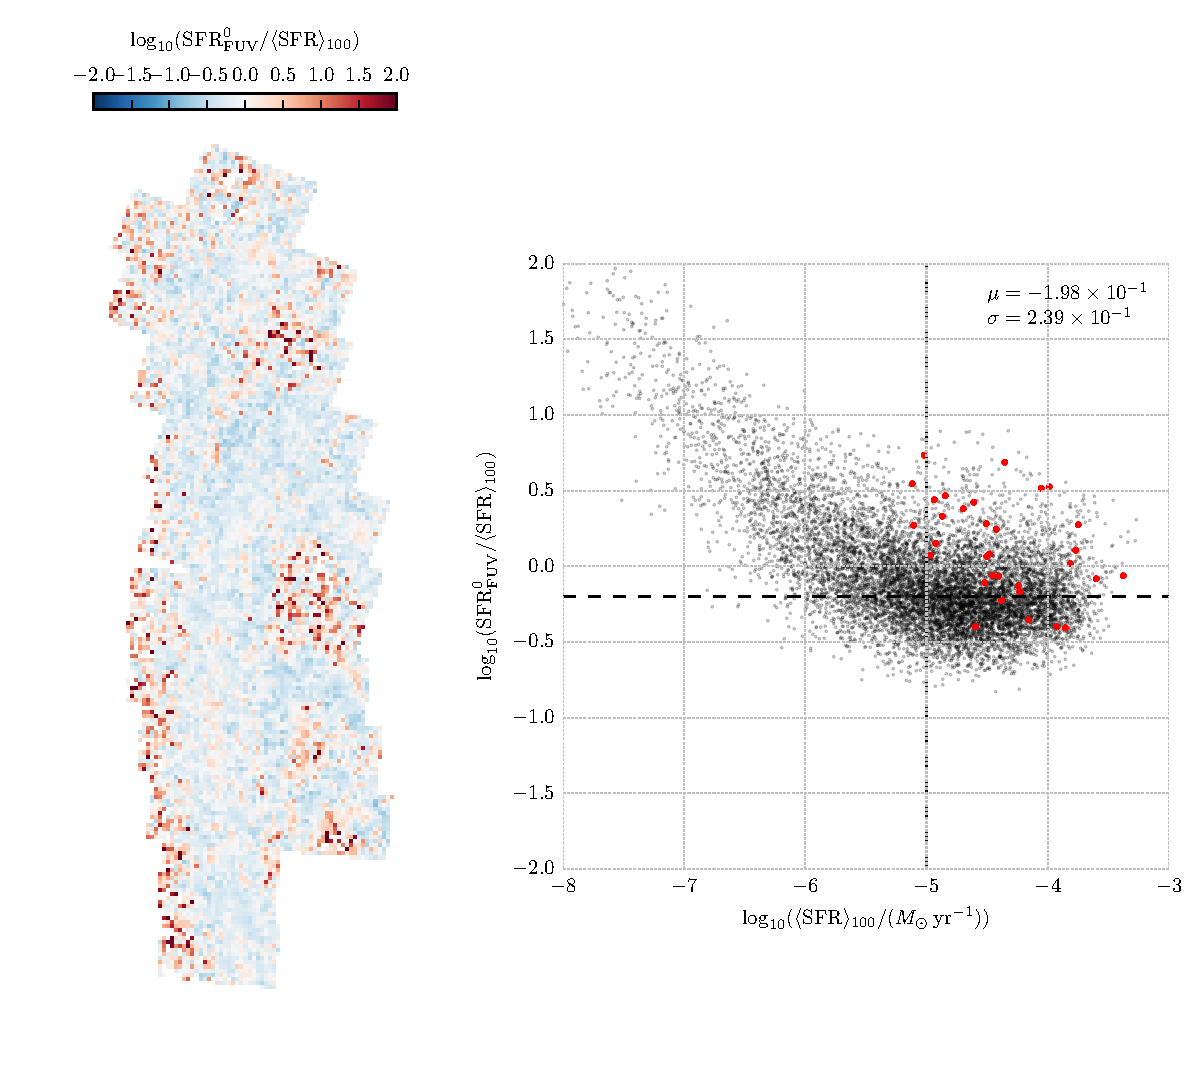
\includegraphics[width=\textwidth]{m31flux-figures/sfr_fuv0-vs-mean.pdf}
\caption[Ratio of the \sfr{} based on the synthetic intrinsic \fuv{} flux to
the $100\myr$ mean \sfr{}.]{Same as Figure \ref{fig:mfx:fuvsfrratio}, but based
    on synthetic instrinsic flux, \sfrfuvz{}. The log-normal distribution is
    characterized by $\mu = -1.98\times 10^{-1}$ and $\sigma = 2.39\times
    10^{-1}$. The median ratio is 0.63 with 68\% confidence limits of 0.37 and
    1.10. \sfrfuvz{} and \sfroneh{} are therefore consistent on average. The
    results here are similar to Figure \ref{fig:mfx:fuvsfrratio}, suggesting
    that SFH variability does not significantly affect the \sfrfuv{}
    uncertainties.
}
\label{fig:mfx:fuvzsfrratio}
\end{figure*}


% Figure 13
\begin{figure*}
\centering
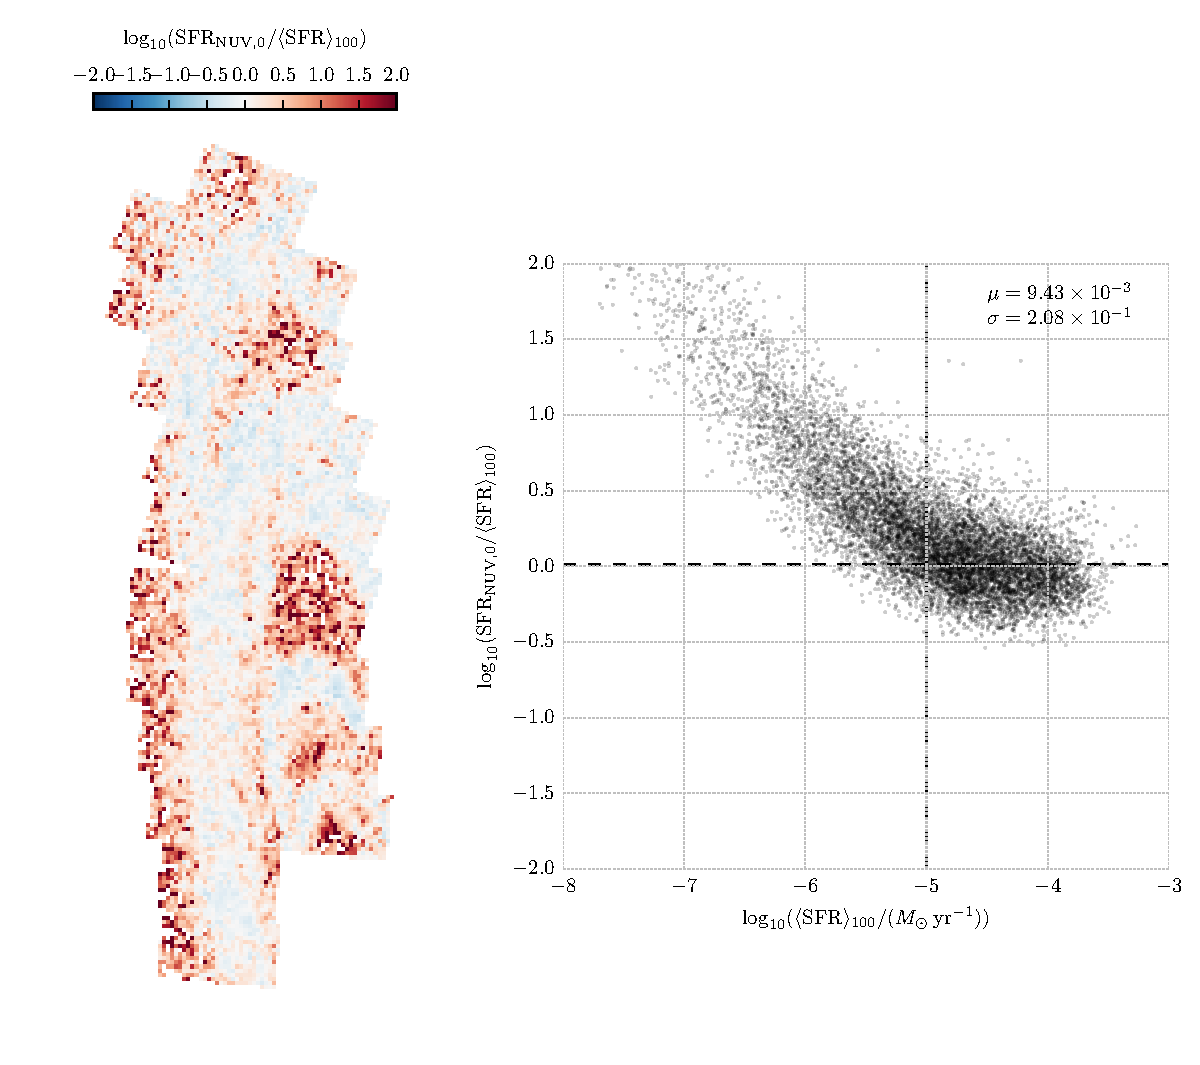
\includegraphics[width=\textwidth]{m31flux-figures/sfr_nuv0-vs-mean.pdf}
\caption[Ratio of the \sfr{} based on the synthetic intrinsic \nuv{} flux to
the $100\myr$ mean \sfr{}.]{Same as Figure \ref{fig:mfx:nuvsfrratio}, but based
    on synthetic instrinsic flux, \sfrnuvz{}. The log-normal distribution is
    characterized by $\mu = 9.43\times 10^{-3}$ and $\sigma = 2.08\times
    10^{-1}$. The median ratio is 1.02 with 68\% confidence limits of 0.63 and
    1.65. \sfrnuvz{} and \sfroneh{} are therefore consistent on average. The
    results here are similar to Figure \ref{fig:mfx:nuvsfrratio}, suggesting
    that SFH variability does not significantly affect the \sfrnuv{}
    uncertainties.
}
\label{fig:mfx:nuvzsfrratio}
\end{figure*}


\sfrxz{} is a useful quantity because it is determined self-consistently.
Converting a SFR (e.g., for an age bin in a SFH) into a flux as demonstrated in
\S \ref{mfx:syntheticfluxmaps:fluxmod} is conceptually the inverse of
converting a flux into a SFR via Equations \ref{mfx:eq:fuvcal} and
\ref{mfx:eq:nuvcal}. Also, both the synthetic fluxes and the flux calibrations
assume a well-sampled IMF from \citet{Kroupa:2001}. The only effect that would
cause a difference between \sfroneh{} and \sfrxz{} for a given SFH is
variability in the SFH itself. We find little difference between the SFR ratio
distributions in Figures \ref{fig:mfx:fuvsfrratio} and
\ref{fig:mfx:fuvzsfrratio} and in Figures \ref{fig:mfx:nuvsfrratio} and
\ref{fig:mfx:nuvzsfrratio}. If SFH variability does play a role in the SFR
ratio variances, then we cannot detect it on a statistically significant basis
and it is therefore not a major contributor to the \sfrx{} and \sfrxz{}
uncertainties.

The \fuv{} SFR ratios from \citet{Simones:2014} are shown in Figures
\ref{fig:mfx:fuvsfrratio} and \ref{fig:mfx:fuvzsfrratio} and appear to follow
the main distributions for the main sample. Comparing the $\mu$ and $\sigma$
values between the two samples, we find that the means are consistent. Part of
the discussion in \citet{Simones:2014} concerned possible explanations for the
apparent overestimation of SFRs relative to \sfroneh{}. However, in the context
of our larger, survey-wide sample we see that the SFR ratios of the UV-bright
regions really are consistent on average.

We do not observe in Figures \ref{fig:mfx:fuvsfrratio},
\ref{fig:mfx:nuvsfrratio}, \ref{fig:mfx:fuvzsfrratio}, or
\ref{fig:mfx:nuvzsfrratio} any environmental trends for the mean or variance of
\sfrx{} and \sfrxz{}, with the exception of the faintest areas of the galaxy
responsible for the tails in the log SFR ratios distributions. Deriving SFRs
from published flux calibrations is therefore generally a safe practice for
environments like M31, \emph{but only as long as the resulting \sfr{}s are
greater than $\sim 10^{-5}\msun\yr^{-1}$}. When applied to sub-kpc regions, we
estimate the resulting uncertainties to be $+\!0.47/\!-\!0.26$ (\fuv{}) and
$+\!0.88/\!-\!0.52$ (\nuv{}) times the true, underlying $100\myr$-mean SFR. The
\sfrfuv{} uncertainty is rather less than the $+\!2.15/\!-\!0.88$ uncertainty
found by \citet{Simones:2014}.

Finally, we evaluate the flux calibrations in Equations \ref{mfx:eq:fuvcal} and
\ref{mfx:eq:nuvcal} for $\sim$galaxy-sized scales, as they are perhaps more
commonly be used, by measuring the global SFR for the entire PHAT survey area.
Summing up all of the pixels in Figure \ref{fig:mfx:sfrmaps1}, we find that
$\sfroneh=0.30\msun\yr^{-1}$, consistent with \citet{Lewis:2014}. In
comparison, the global flux-based SFRs are $0.22\msun\yr^{-1}$ for \fuv{} and
$0.43\msun\yr^{-1}$ for \nuv{}. If we adopt the estimated uncertainties
mentioned earlier in this section, then the global flux-based SFRs are well
within uncertainty of \sfroneh{}. However, as larger areas are considered, IMF
sampling effects should eventually disappear and the variances in the SFR
ratios should correspondingly decrease. Therefore, our estimated uncertainties
should be considered firm upper limits when applied to galaxies. The global SFR
ratios (flux-based to mean) are 0.73 and 1.43 for \fuv{} and \nuv{},
respectively. Why these ratios are larger than the median ratios above is not
yet understood.





\section{Conclusion}\label{mfx:conclusion}

We have used star formation histories (SFHs) to model the spectral energy
distributions (SEDs) of over 9000 sub-kpc regions in M31 and produce detailed
maps of synthetic UV flux across the entire area covered by the Panchromatic
Hubble Andromeda Treasury (PHAT). This work is an extensive follow-up to the
analysis of \citet{Simones:2014}, which involved only 33 ultraviolet
(UV)-bright regions from a small portion of the galaxy. The SFHs were derived
by \citet{Lewis:2014}\ using \acsb{} and \acsi{} photometry from the PHAT
survey. Both intrinsic and attenuated SEDs were derived from the SFHs using the
Flexible Stellar Population Synthesis (FSPS) code. These were convolved with
the Galaxy Evolution Explorer (GALEX) \fuv{} and \nuv{} response curves to
obtain the synthetic intrinsic fluxes, \fxsfhz{}, as well as the synthetic
attenuated fluxes, \fxsfh{}. All of the flux values were then assembled into an
overall map, or mosaic, using Montage. The mosaic pixels corresponded to
physical areas of $4.4\times 10^4\pc^2$. We constructed corresponding maps for
the observed flux, \fxobs{}, using GALEX Deep Imaging Survey (DIS) images.

The \fxsfh{} maps agreed with the \fxobs{} maps very well with respect to the
broad morphology of M31, faithfully reproducing all of the main features
brighter than $\sim 10^{-15}\uflambda$. We found the log ratios of \fxsfh{} to
\fxobs{} to be log-normally distributed with $\mu = 7.62\times 10^{-3}$ and
$\sigma = 2.37\times 10^{-1}$ for \fuv{}, and $\mu = -1.03\times 10^{-1}$ and
$\sigma = 1.59\times 10^{-1}$ for \nuv{}. The median flux ratios were 1.02 in
\fuv{} and 0.79 in \nuv{}, with 68\% confidence limits of 0.59 and 1.76
(\fuv{}) and 0.55 and 1.14 (\nuv{}). In both filters, the median ratio was
within the confidence interval of 1, indicating that \fxsfh{} was consistent
with \fxobs{} on average. Due to the small pixel areas, the primary source of
the variance in the log flux ratios was most likely related to incomplete
sampling of the IMF.

We found no obvious trends in the flux ratios with respect to environment,
except for in the faintest, off-arm areas of the M31 where the variances in the
flux ratios were noticeably larger. We conclude that fluxes may be successfully
modeled from SFHs for any population in environments similar to M31. For our
sub-kpc regions, we estimate the synthetic flux uncertainties to be
$+\!0.74/\!-\!0.43$ and $+\!0.35/\!-\!0.24$ in \fuv{} and \nuv{}, respectively.
Results from previous work on UV-bright regions by \citet{Simones:2014} were
consistent with our results.

The overall agreement between the observed and synthetic fluxes is remarkable
considering that our flux modeling procedure was dependent on several key
assumptions. Specifically, we assumed an IMF, models describing stellar spectra
and evolution, and an extinction model as well as an extinction curve. These
form the foundation for much research in astronomy and encompass our current
best understanding of stellar astrophysics and star formation. It is reassuring
that we can use all of this knowledge to successfully recreate detailed maps of
a galaxy from photometry in just two optical bands.

We used flux calibrations from \citet{Kennicutt:1998} with updates by
\citet{Hao:2011} and \citet{Murphy:2011} to estimate SFRs based on observed UV
flux, \sfrx{}. The \fxobs{} maps were first corrected for extinction using the
synthetic attenuated and intrinsic fluxes. We also calculated the $100\myr$
mean SFR from the SFHs, \sfroneh{}. We found that the faintest areas of M31 had
the highest ratios of \sfrx{} to \sfroneh{} and formed a linear tail feature in
plots of the SFR ratio versus \sfroneh{}. These tails were the result of a
distinct breakdown of the linear relationship between flux and SFR which
underpins the flux calibration method. We estimated a conservative threshold of
$\sfr \sim 10^{-5}\msun\yr^{-1}$ below which flux calibration should not be
used.

For the pixels above this threshold, we found the SFR ratios to be log-normally
distributed with $\mu = -2.46\times 10^{-1}$ and $\sigma = 2.61\times 10^{-1}$
for \fuv{}, and $\mu = 9.27\times 10^{-2}$ and $\sigma = 2.33\times 10^{-1}$
for \nuv{}. The median ratios are 0.57 (\fuv{}) and 1.24 (\nuv{}), with 68\%
confidence limits of 0.31 and 1.04 (\fuv{}) and 0.72 and 2.12 (\nuv{}),
indicating that \sfrx{} is consistent with \sfroneh{} on average. As with the
flux ratios, incomplete sampling of the IMF was the main source of the variance
in the SFR ratios. We also considered deviations from solar metallicity as well
as SFH variability, and found that they were far less important for the overall
variances in the SFR ratios than IMF sampling.

Other than the faintest, off-arm areas which responsible for the tail feature
in the SFR ratio distributions, there were no found no obvious trends in the
SFR ratios with respect to environment. We determine that the flux calibration
method is safely applicable to environments similar to M31, \emph{but only as
long as the resulting \sfr{}s are greater than $\sim 10^{-5}\msun\yr^{-1}$}. We
estimate the SFR uncertainties for our sub-kpc regions to be
$+\!0.47/\!-\!0.26$ (\fuv{}) and $+\!0.88/\!-\!0.52$ (\nuv{}) times the true,
underlying $100\myr$-mean SFR. The \sfrfuv{} uncertainty is rather less than
the $+\!2.15/\!-\!0.88$ uncertainty previously found by \citet{Simones:2014}.

We also measured global SFRs for the entire PHAT survey area. The global
\sfroneh{} value was $0.30\msun\yr^{-1}$, while the UV flux-based values were
$\sfrfuv = 0.22\msun\yr^{-1}$ and $\sfrnuv = 0.43\msun\yr^{-1}$. The flux-based
global SFRs are consistent with the global \sfroneh{} value to within the
uncertainties derived from the SFR maps. However, the variances in the SFR
ratios due to IMF sampling is expected to decrease for larger areas, so our
estimated uncertainties should be considered firm upper limits when applied to
galaxies. The global SFR ratios (flux-based to mean) are 0.73 and 1.43 for
\fuv{} and \nuv{}, respectively. Why these ratios are larger than the median
ratios above is not yet understood.

This research has made use of NASA's Astrophysics Data System Bibliographic
Services and the NASA/IPAC Extragalactic Database (NED), which is operated by
the Jet Propulsion Laboratory, California Institute of Technology, under
contract with the National Aeronautics and Space Administration. This work was
supported by the Space Telescope Science Institute through GO-12055. Support
for D.~R.~W is provided by NASA through Hubble Fellowship grant HST-HF-51331.01
awarded by the Space Telescope Science Institute, which is operated by the
Association of Universities for Research in Astronomy, Inc., under NASA
contract NAS 5-26555. This research made use of Astropy, a community-developed
core Python package for Astronomy \citep{Astropy_Collaboration:2013}, as well
as NumPy and SciPy \citep{Oliphant:2007}, IPython \citep{Perez:2007}, and
Matplotlib \citep{Hunter:2007}. This research made use of Montage, funded by
the National Aeronautics and Space Administration's Earth Science Technology
Office, Computation Technologies Project, under Cooperative Agreement Number
NCC5-626 between NASA and the California Institute of Technology. Montage is
maintained by the NASA/IPAC Infrared Science Archive.





\bibliographystyle{apj}  % apj.bst
\bibliography{references}

\end{document}
